\documentclass[hidelinks,aspectratio=169]{beamer}
\usepackage[italian]{babel} 
\usepackage[utf8]{inputenc} 
\usepackage{fourier} 


%Slide colors
\usetheme{Boadilla}
\usecolortheme{beaver}

% Images
\usepackage{graphicx}
\usepackage{caption}
\usepackage{subcaption}
\usepackage{float}
\graphicspath{ {../Images} }

% FlowChart
\usepackage{smartdiagram}

% Stop hyphenation
\usepackage[none]{hyphenat}

% Coloring links
\usepackage{xcolor}

% Enumerate abc
\usepackage{enumerate}

% Minipages in the same line
\usepackage{tabularx}

% Redefines caption setup in way to remove "Figure:"
\usepackage{caption}
\captionsetup[figure]{labelformat=empty}

% License
\usepackage[
type={CC},
modifier={by-nc-sa},
version={4.0},
]{doclicense}

% Command to enumerate frames title
\newcommand{\numcirc}[1]{%
	%   \usebeamerfont*{item projected}%
	\large
	\usebeamercolor[bg]{item projected}%
	\begin{pgfpicture}{-1ex}{0ex}{1ex}{2ex}
		\pgfpathcircle{\pgfpoint{0pt}{.75ex}}{1.2ex}
		\pgfusepath{fill}
		\pgftext[base]{\color{fg}#1}
	\end{pgfpicture}%
	\usebeamerfont*{frametitle}%
}

%Command to zoom in
\usepackage{mwe}
\makeatletter
\newsavebox\zb@x
\newcounter{z@@m}
\usepackage{calc}
\newdimen\B@r\newdimen\P@r
\newdimen\@zw\newdimen\@zh\newdimen\@zd

\newcommand{\zoombox}[2][0]{%
	\leavevmode%
	\sbox\zb@x{#2}%
	\setlength\B@r{1pt*\ratio{\wd\zb@x}{\ht\zb@x+\dp\zb@x}}%
	\setlength\P@r{1pt*\ratio{\paperwidth}{\paperheight}}%
	\ifdim\B@r>\P@r\relax%
	\setlength\@zw{\wd\zb@x}\setlength\@zh{\@zw*\ratio{\paperheight}{\paperwidth}}%
	\setlength\@zd{(\@zh-\ht\zb@x-\dp\zb@x)*\real{0.5}+\dp\zb@x}%
	\setlength\@zh{\@zh-\@zd}%
	\else%
	\setlength\@zh{\ht\zb@x+\dp\zb@x}%
	\setlength\@zw{\@zh*\ratio{\paperwidth}{\paperheight}}%
	\setlength\@zh{\ht\zb@x}\setlength\@zd{\dp\zb@x}%
	\fi%
	\makebox[0pt][l]{\makebox[\wd\zb@x][c]{\makebox[\@zw][l]{%
				\pdfdest name {zbfs\thez@@m} fitr
				width  \@zw\space
				height \@zh\space
				depth  \@zd\space
	}}}%
	\pdfdest name {zb\thez@@m} fitr
	width  \wd\zb@x\space
	height \ht\zb@x\space
	depth  \dp\zb@x\space
	\immediate\pdfannot 
	width  \wd\zb@x\space
	height \ht\zb@x\space
	depth  \dp\zb@x\space
	{%
		/Subtype/Link/H/N
		/Border [0 0 #1 [1 2]]
		/A <<
		/S/JavaScript
		/JS (
		if(typeof(zoomed)=='undefined'||!zoomed){
			var lastView=this.viewState;
			if(app.fs.isFullScreen) this.gotoNamedDest('zbfs\thez@@m');
			else this.gotoNamedDest('zb\thez@@m');
			zoomed=true;
		}else{
			this.viewState=lastView;
			zoomed=false;
		}
		)
		>>
	}%
	\usebox{\zb@x}%
	\stepcounter{z@@m}%
} 
\makeatother



%Header
\title[Identità e valore della stampa d'arte]{\textbf{Identità e valore della stampa d'arte}}
\author{Roberto Budassi}
\date{}

\begin{document}
	
		\begin{frame}
		\maketitle
		
		\vspace*{\fill}
		\centering
		\fboxrule=2pt
		\fbox
		{
			\begin{minipage}{0.9\linewidth}
				\small{Il seguente documento è ottimizzato per la visualizzazione digitale con \href{https://get.adobe.com/it/reader/}{\textcolor{blue}{Adobe~Acrobat~Reader}}.}  
			\end{minipage}
		}
	\end{frame}
	
	\begin{frame}
		\tableofcontents
	\end{frame}
	
	\section{Sul concetto di \textbf{originalità} e \textbf{autenticità}}
	\begin{frame}{Sul concetto di \textbf{originalità} e \textbf{autenticità}}
		\begin{itemize}
			\item 1937	Parigi: Exposition Internationale - Comité National de la Gravure
			\item 1960	Vienna: 3° Congresso - Associazione Internazionale delle Arti Plastiche
			\item 1961	New York: Print Council of America
			\item 1964	Parigi: Comité International de la Gravure
			\item 1991	Venezia: convegno organizzato dalla Biennale di Venezia
			\item 1994	Milano: dichiarazione sull’incisione originale
		\end{itemize}
	\end{frame}
	
	\begin{frame}{Sul concetto di \textbf{originalità} e \textbf{autenticità}}
		In sintesi….“Un’incisione è considerata “originale” quando rispetta le due seguenti caratteristiche:
		\begin{enumerate}[a.]
			\item In fase di stampa dà luogo a un’immagine che deriva da una matrice manualmente incisa (anche nel caso in cui l’artista si sia servito di una base ottenuta con altri procedimenti), o predisposta sempre manualmente dallo stesso artista, con esclusione di qualsiasi mezzo fotomeccanico, allo scopo di essere impressa con intenti estetici.
			\item L’immagine incisa sulla matrice deve seguire la sintassi linguistica propria dell'incisione, e cioè un appropriato e intenzionale uso delle tecniche specifiche.
		\end{enumerate}
		Per analogia una litografia viene considerata “stampa originale” quando la sua immagine è impressa da una matrice manualmente disegnata o dipinta, allo scopo di essere stampata con intenti estetici.\\
		Qualunque stampa che riproduca un modello, ottenuta con mezzi fotomeccanici, o con altri mezzi non manuali, di qualsivoglia tipo, non può essere chiamata “originale” (e neppure “originaria” o “litografia autentica”).
	\end{frame}
	
	\subsection{Le tecniche originali}
	\begin{frame}{Le tecniche originali}
		Stampa in rilievo (xilografia), in incavo (calcografia), in piano (litografia)
		\begin{tabularx}{\textwidth}{XXX}
			{
			\begin{center}
				\large{Xilografia}\\
				\bigskip
				\begin{itemize}
					\item \small{\textbf{Bulino} su legno di filo}
					\item \small{\textbf{Bulino} su legno di testa}
					\item \small{\textbf{Camaieu}}
					\item \small{\textbf{Criblèe} su metallo}
					\item \small{\textbf{Sgorbia} su linoleum}
					\item \small{\textbf{Sgorbia} su cartone}
				\end{itemize}
			\end{center}
			}&{
			\begin{center}
				\large{Calcografia}\\
				\normalsize
				\bigskip
				\normalsize{(Maniera diretta)}\\
				\begin{itemize}
					\item \scriptsize{\textbf{Niello}}
					\item \scriptsize{\textbf{Bulino}}
					\item \scriptsize{\textbf{Puntasecca}}
					\item \scriptsize{\textbf{Mezzotinto/Maniera nera}}
					\item \scriptsize{\textbf{Carborundum}}
				\end{itemize}
				\medskip
				\normalsize{(Maniera indiretta)}\\
				\begin{itemize}
					\item \scriptsize{\textbf{Acquaforte}}
					\item \scriptsize{\textbf{Acquatinta}}
					\item \scriptsize{\textbf{Maniera a zucchero}}
					\item \scriptsize{\textbf{Vernice molle}}
				\end{itemize}
			\end{center}
			}&{
			\begin{center}
				\large{Litografia}\\
				\normalsize
				\bigskip
				\begin{itemize}
					\item \small{\textbf{Su matrice di pietra}}
					\item \small{\textbf{Su matrice di zinco}}
					\item \small{\textbf{Cromolitografia}}
				\end{itemize}
			\end{center}
			}
		\end{tabularx}
	\end{frame}
	
	\begin{frame}{Le tecniche originali}
		\begin{tabularx}{\textwidth}{XXX}
			{
			\centering
			\zoombox{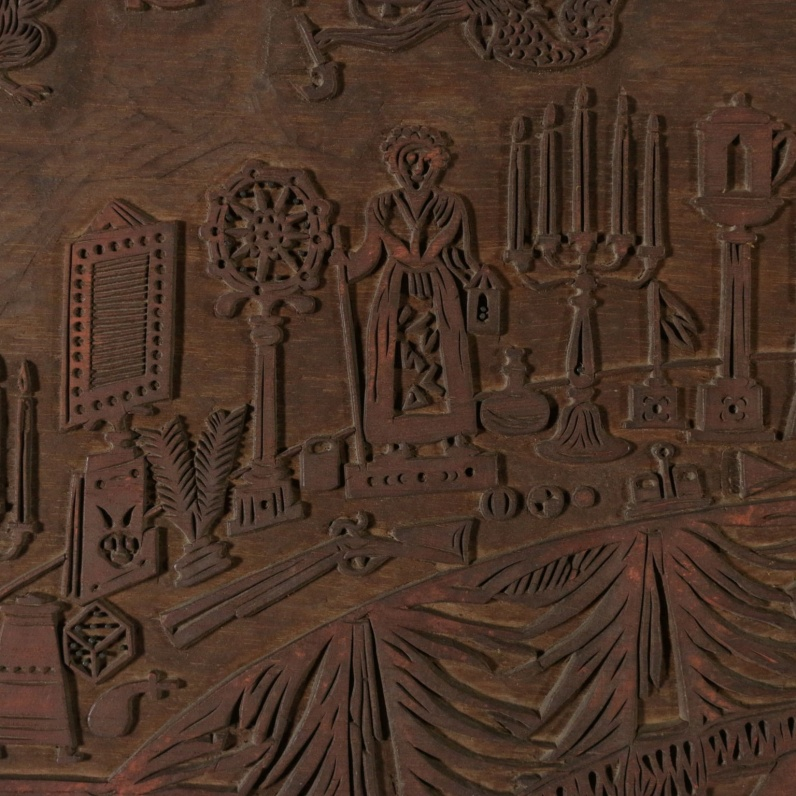
\includegraphics[scale=0.5]{Esempio1.jpg}}
			\captionof{figure}{Matrice xilografica}
			}&{
			\centering
			\zoombox{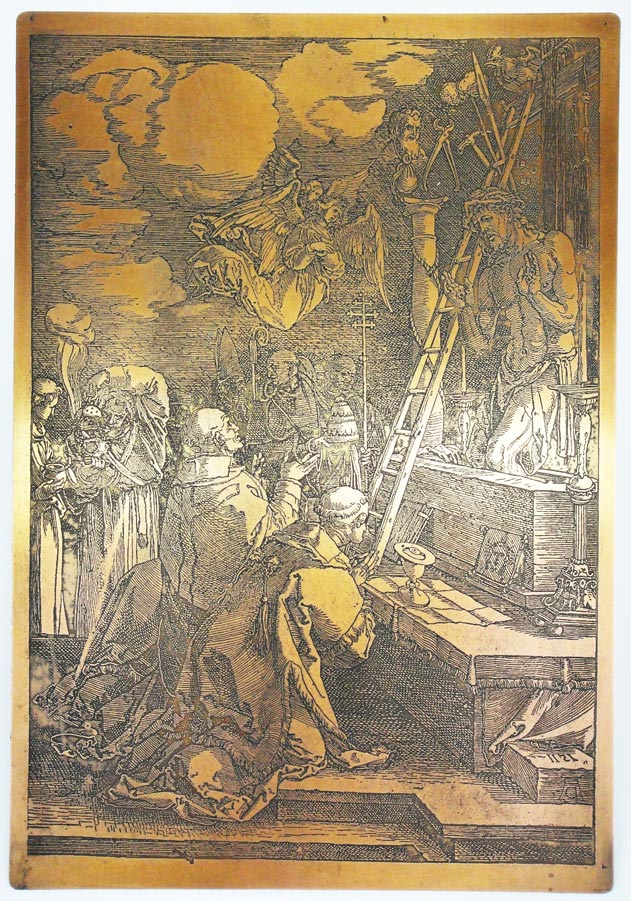
\includegraphics[scale=0.15]{Esempio2.jpg}}
			\captionof{figure}{Matrice  incavografica}
			}&{
			\centering
			\zoombox{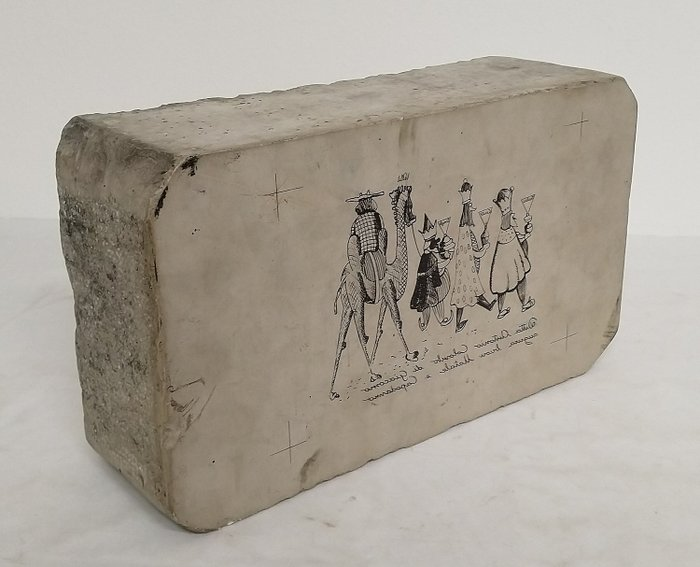
\includegraphics[scale=0.17]{Esempio3.jpg}}
			\captionof{figure}{Matrice litografica}
			}
		\end{tabularx}
	\end{frame}
	
	\begin{frame}{Le tecniche originali}
		\begin{tabularx}{\textwidth}{XXX}
			{
			\centering
			\zoombox{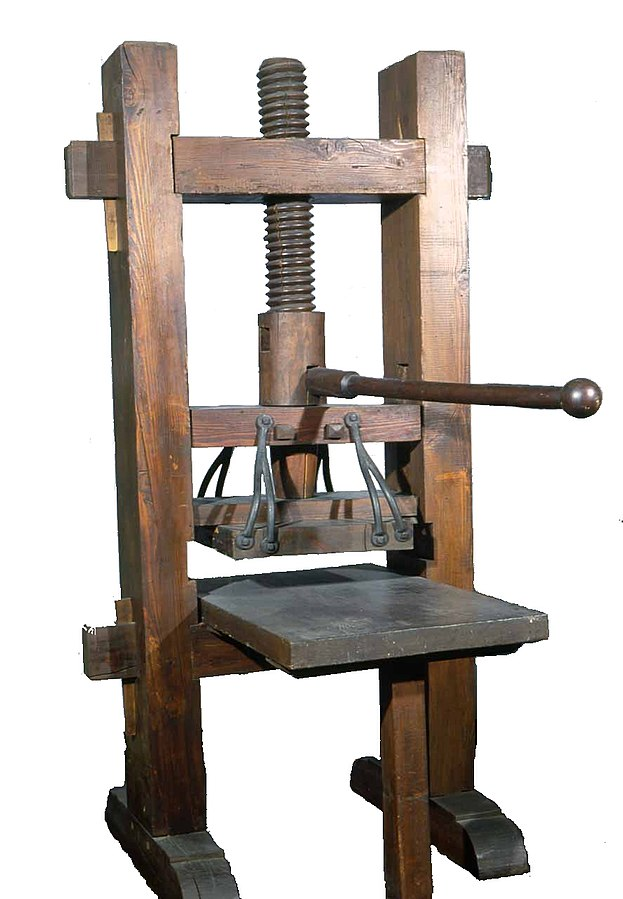
\includegraphics[scale=0.13]{Macchina1.jpg}}
			%\captionof{figure}{Esempio 1}
			\zoombox{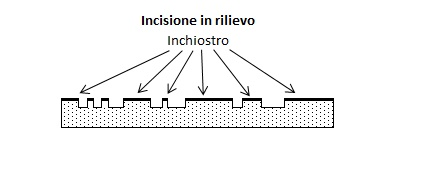
\includegraphics[scale=0.5]{Macchina11.jpg}}
			\captionof{figure}{Stampa xilografica}
			}&{
			\centering
			\hspace{2mm}
			\zoombox{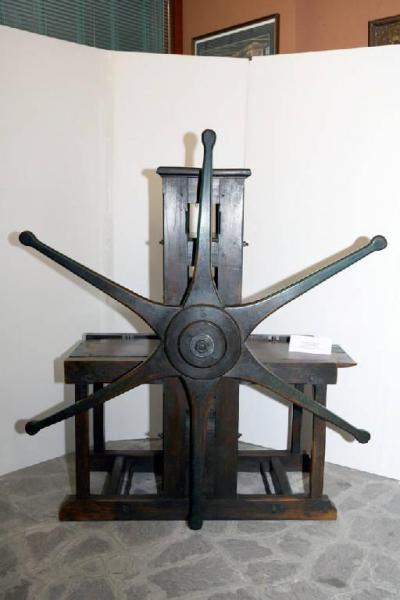
\includegraphics[scale=0.25]{Macchina2.jpg}}
			%\captionof{figure}{Esempio 1}
			\vspace*{3mm}
			\zoombox{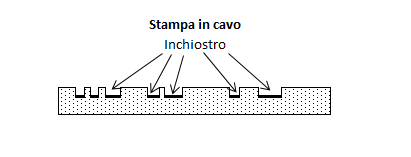
\includegraphics[scale=0.5]{Macchina22.png}}
			\captionof{figure}{Stampa in incavo}
			}&{
			\centering
			\zoombox{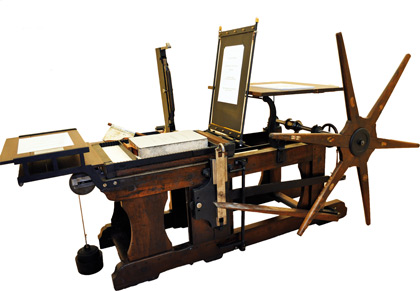
\includegraphics[scale=0.33]{Macchina3.jpg}}
			%\captionof{figure}{Esempio 1}
			\vspace{3mm}
			\zoombox{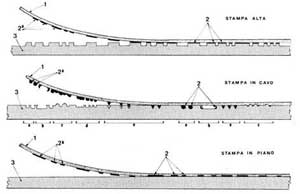
\includegraphics[scale=0.3]{Macchina33.jpg}}
			\captionof{figure}{Stampa litografica}
			}
		\end{tabularx}
	\end{frame}
	
	\begin{frame}{Le tecniche originali}
		\begin{tabularx}{\textwidth}{XXX}
			{
			\centering
			\zoombox{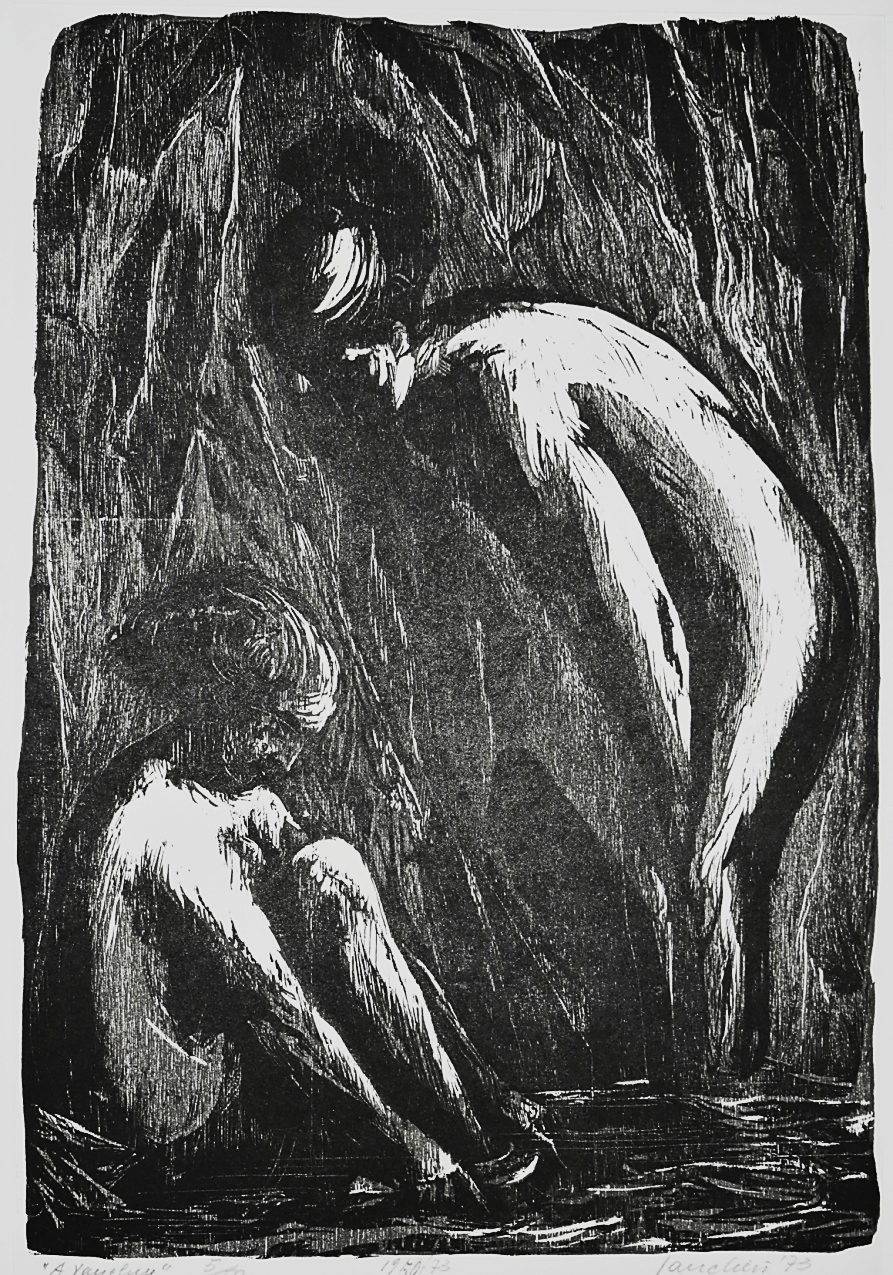
\includegraphics[scale=0.3]{Pietro Sanchini, xilografia.png}}
			\captionof{figure}{\centering Pietro Sanchini, xilografia}
			}&{
			\centering
			\hspace*{-7mm}
			\zoombox{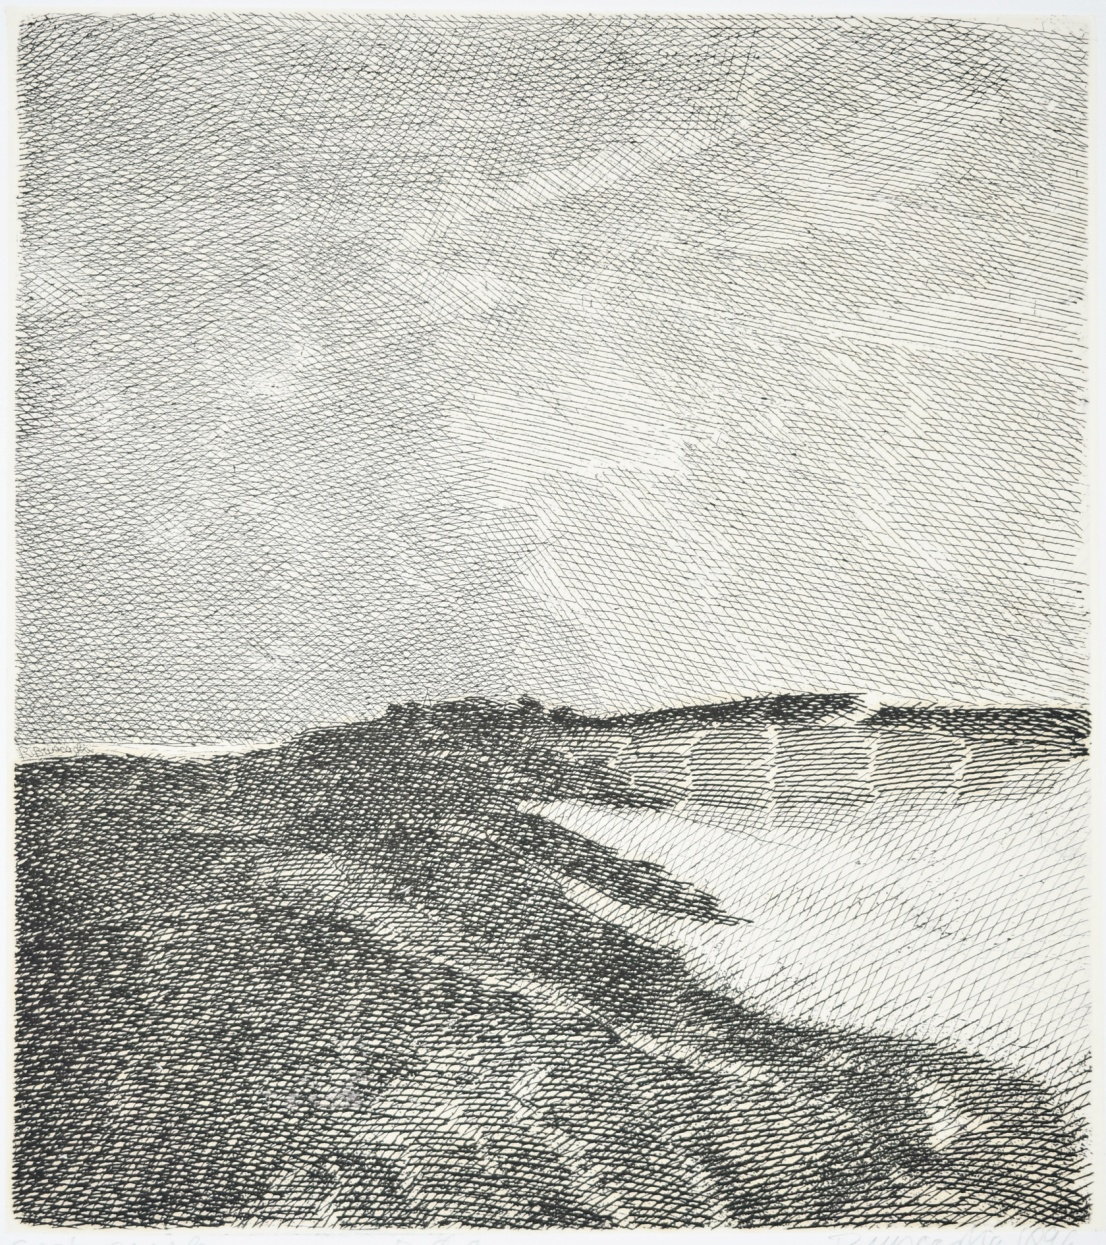
\includegraphics[scale=0.3]{Renato Bruscaglia, acquaforte.jpg}}
			\captionof{figure}{\centering \hspace*{-7mm} Renato Bruscaglia, acquaforte}
			}&{
			\centering
			\zoombox{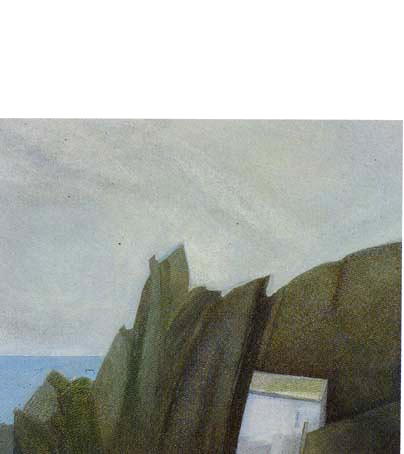
\includegraphics[scale=0.3]{Carlo Ceci, litografia.png}}
			\captionof{figure}{\centering Carlo Ceci, litografia}
			}
		\end{tabularx}
	\end{frame}
	
	\subsection{La stampa di traduzione}
	\begin{frame}{La stampa di traduzione (autografa)}
		\begin{tabularx}{\linewidth}{XX}
			{
			\centering
			\hspace{10mm}
			\zoombox{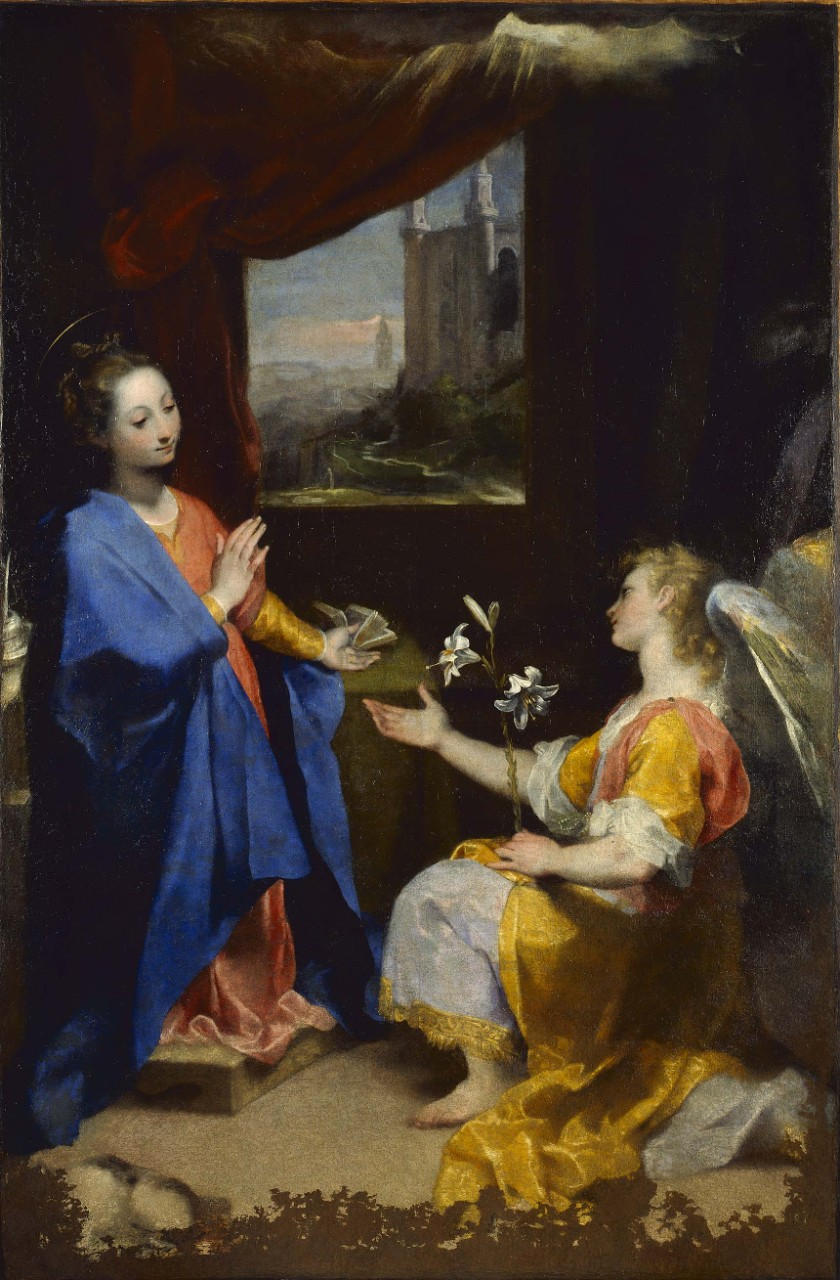
\includegraphics[scale=0.14]{Federico Barocci, Annunciazione, olio su tela.jpg}}
			}&{
			\centering
			\hspace{10mm}
			\zoombox{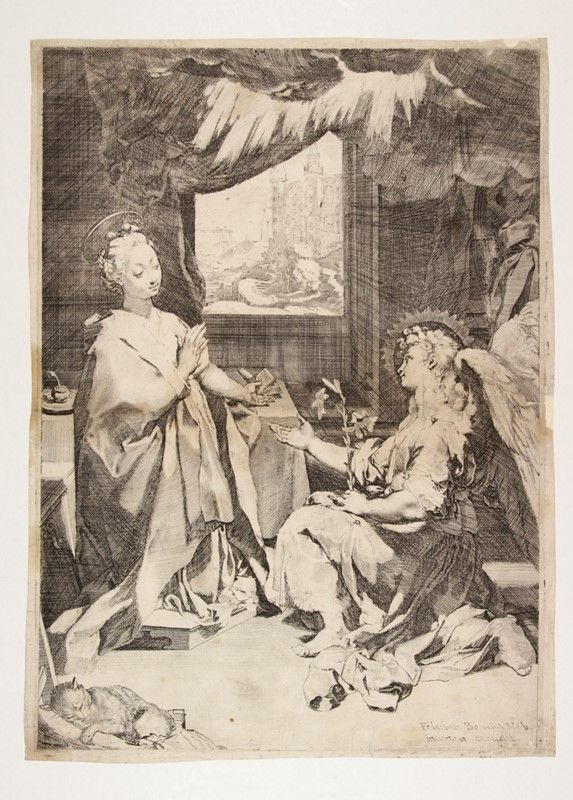
\includegraphics[scale=0.23]{Federico Barocci, Annunciazione, bulino-acquaforte.jpg}}
			}
		\end{tabularx}
		%\hspace*{8mm}
		\centering
		\small{Federico Barocci, Annunciazione, olio su tela – bulino/acquaforte.}
	\end{frame}
	
	\begin{frame}{La stampa di traduzione}
		\vspace*{3mm}
		\begin{tabularx}{\linewidth}{XX}
			{
			\centering
			\zoombox{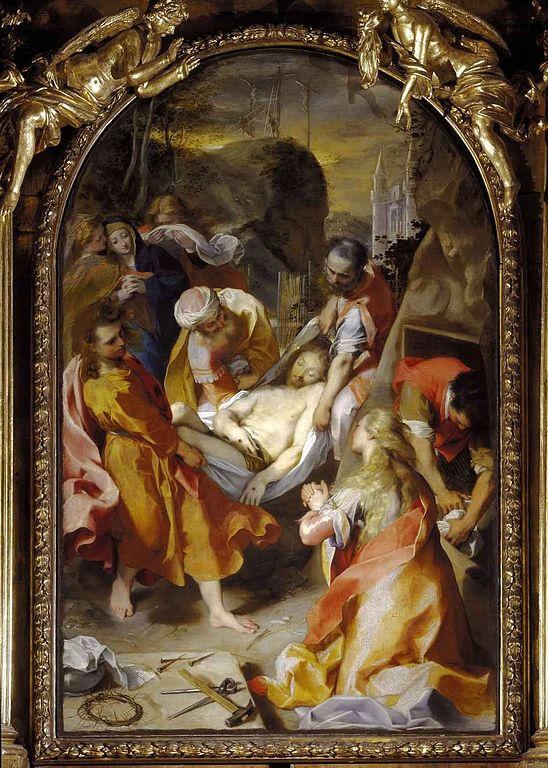
\includegraphics[scale=0.28]{Federico Barocci, Deposizione, olio su tela.jpg}}
			\captionof{figure}{\centering Federico Barocci, Deposizione, olio su tela}
			}&{
			\centering
			%\vspace*{-15mm}
			\zoombox{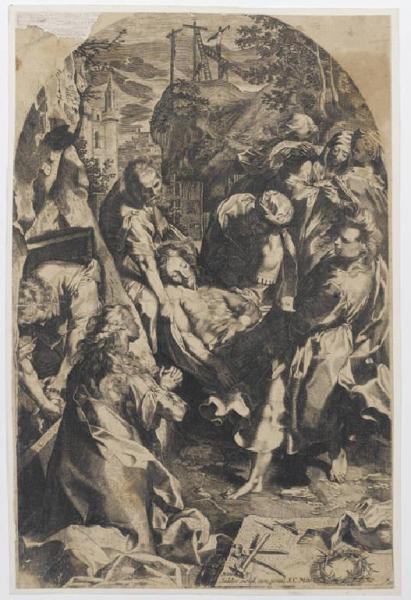
\includegraphics[scale=0.35]{Egidius Sadeler, Deposizione da Brocci, bulino-acquaforte.jpg}}
			\captionof{figure}{\centering Egidius Sadeler, Deposizione da Brocci, bulino/acquaforte}
			}
		\end{tabularx}
	\end{frame}
	
	\begin{frame}{La stampa di traduzione}
		\begin{tabularx}{\linewidth}{XX}
			{
			\hspace*{4mm}
			\centering
			\zoombox{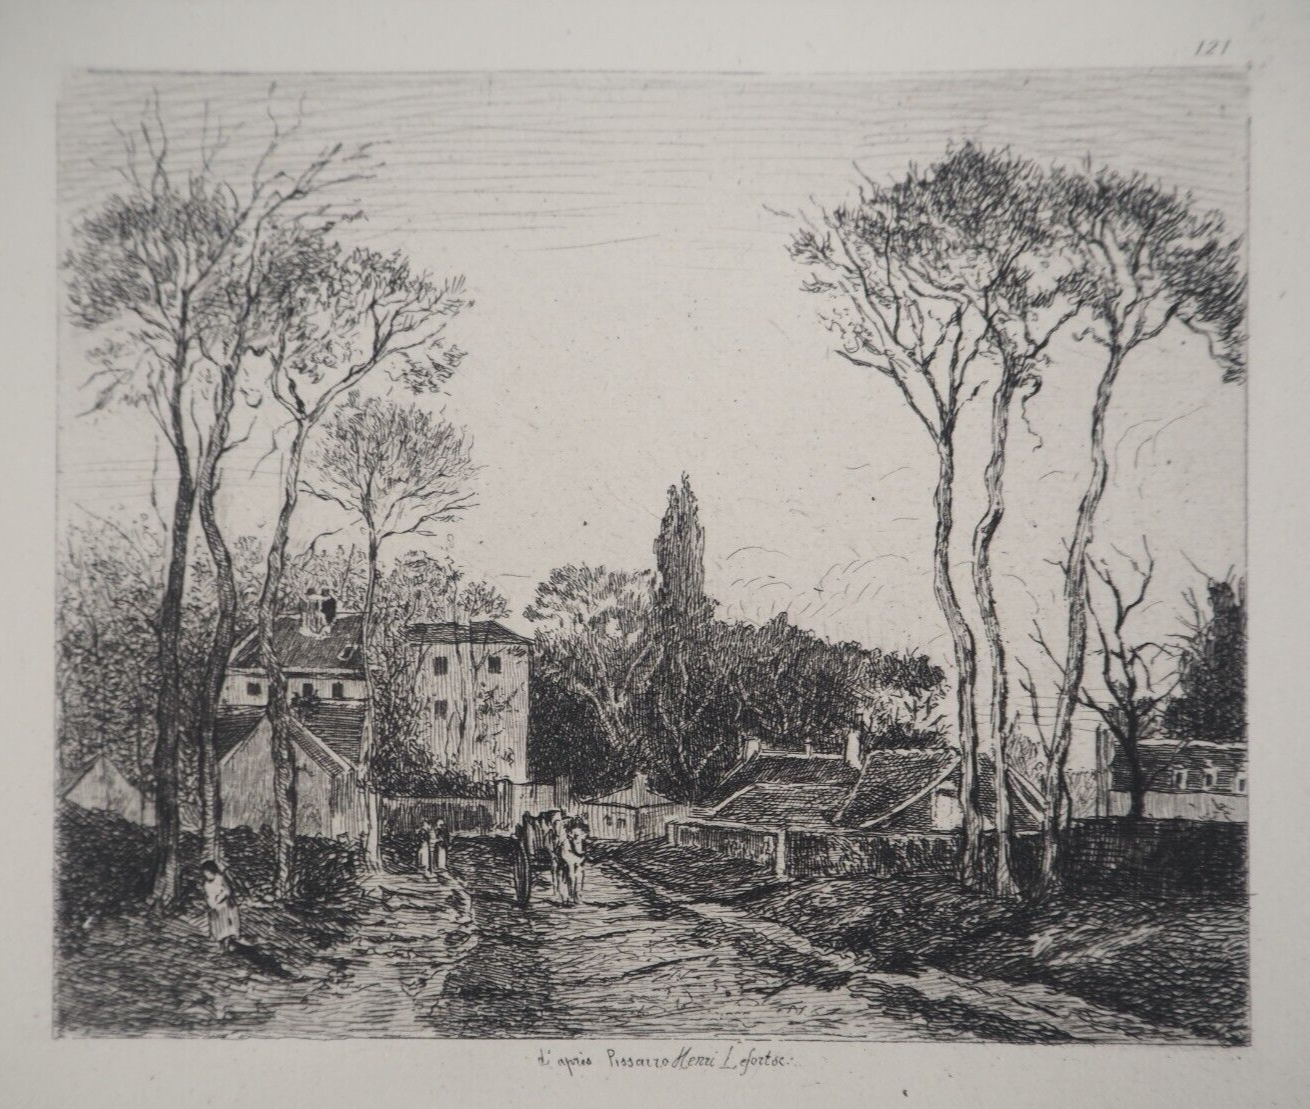
\includegraphics[scale=0.13]{Durand Ruel1.png}}
			}&{
			\hspace*{4mm}
			\centering
			\zoombox{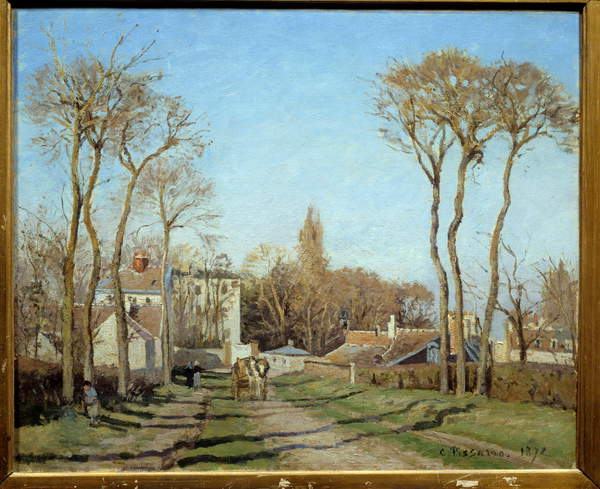
\includegraphics[scale=0.3]{Durand Ruel2.jpg}}
			}		
		\end{tabularx}
		%\vspace*{2mm}
		\centering
		\small{Durand Ruel, Strada vicino Voisin, da Camille Pissarro, olio su tela, 1873}
	\end{frame}
	
	\subsection{La stampa di invenzione}
	\begin{frame}{La stampa di invenzione}
		\begin{tabularx}{\linewidth}{X}
			\centering
			\vspace*{2mm}
			\zoombox{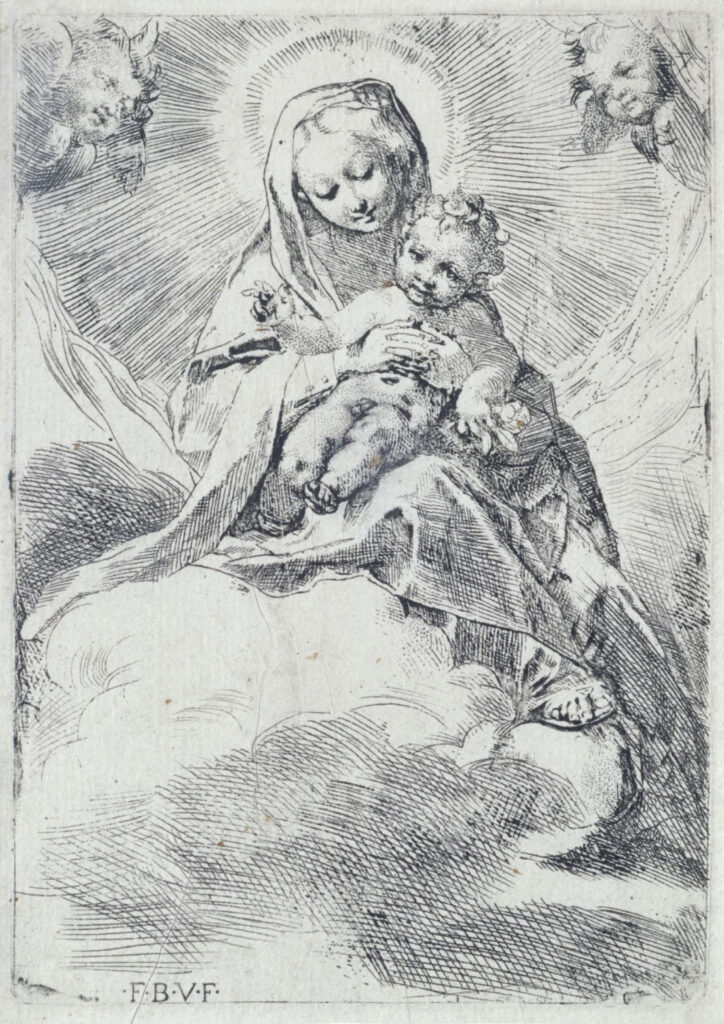
\includegraphics[scale=0.17]{Federico Barocci, Madonna delle nuvole, acquaforte e bulino.jpg}}
			\captionof{figure}{\centering Federico Barocci, Madonna delle nuvole, acquaforte e bulino}
		\end{tabularx}
	\end{frame}
	
	\begin{frame}{La copia}
		\begin{tabularx}{\linewidth}{XXX}
			{
			\centering
			\hspace*{2mm}
			\zoombox{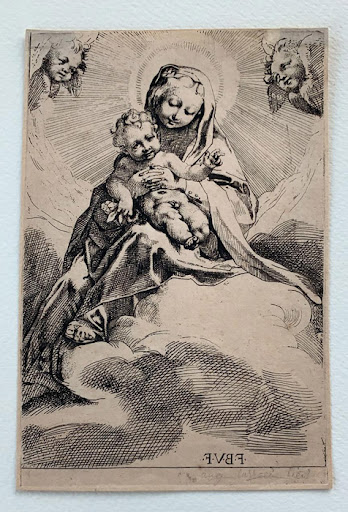
\includegraphics[scale=0.35]{Madonna1.jpg}}
			}&{
			\centering
			\zoombox{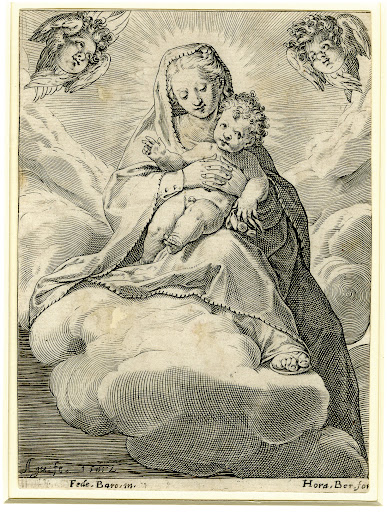
\includegraphics[scale=0.35]{Madonna2.jpg}}
			}&{
			\centering
			\zoombox{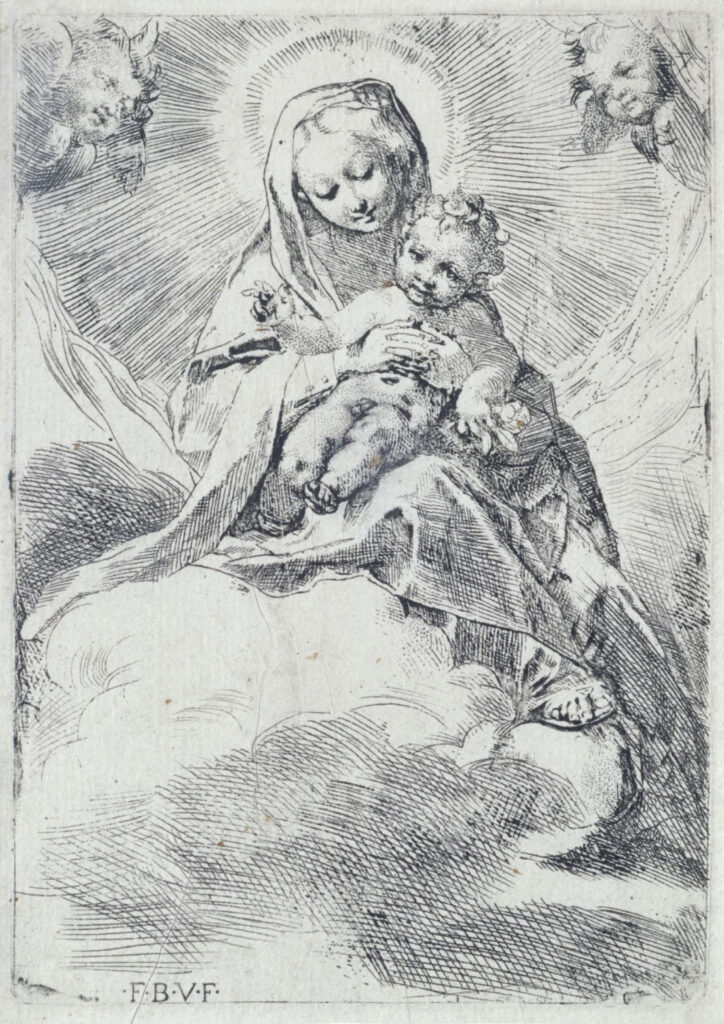
\includegraphics[scale=0.173]{Madonna3.jpg}}
			}
		\end{tabularx}
		\centering
		\small{Autore ignoto e Agostino Carracci, Madonna delle nuvole, copie da Federico Barocci, bulino/acquaforte}
	\end{frame}
	
	\begin{frame}{Stampa di invenzione}
		\begin{tabularx}{\linewidth}{XX}
			{
			\centering
			\hspace*{3mm}
			\zoombox{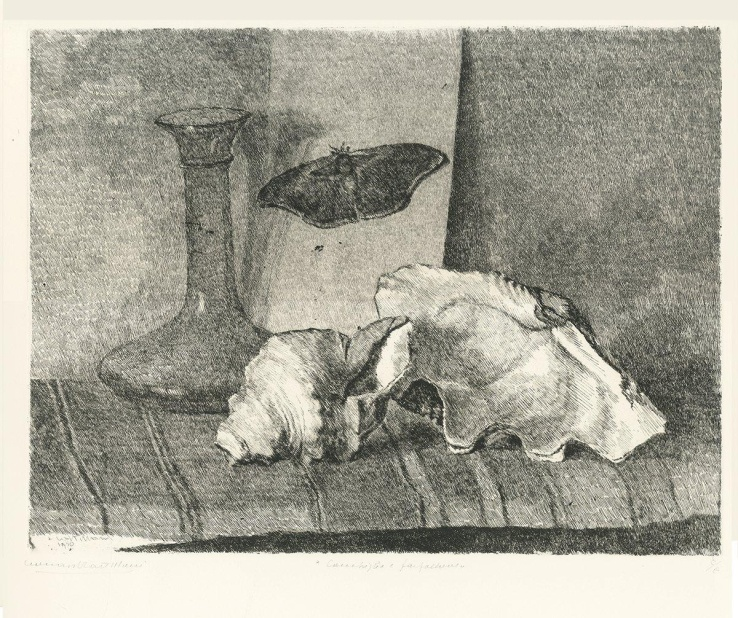
\includegraphics[scale=0.8]{Leonardo Castellani1.jpg}}
			}&{
			\centering
			\hspace*{12mm}
			\zoombox{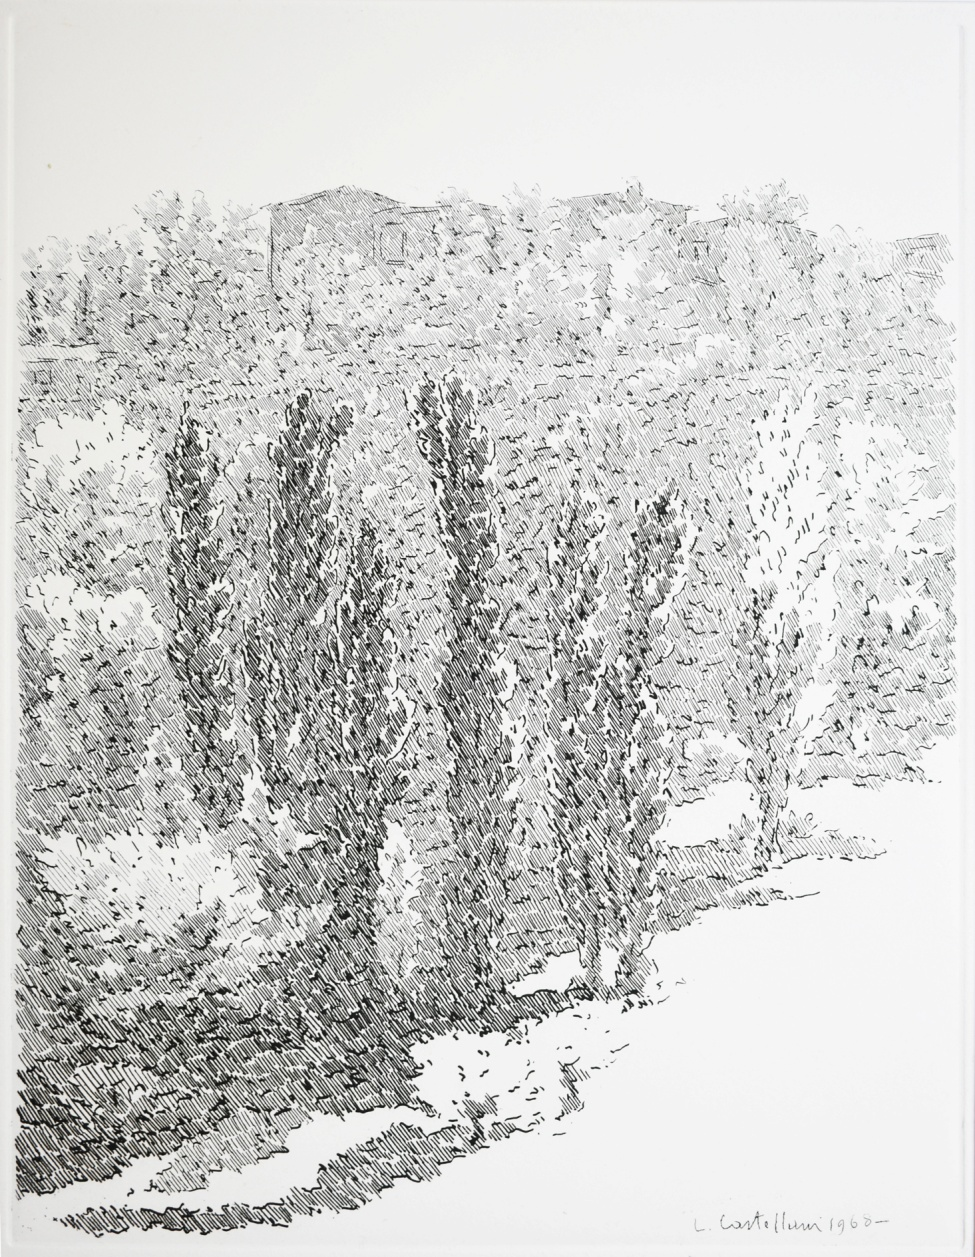
\includegraphics[scale=0.4]{Leonardo Castellani2.jpg}}
			}
		\end{tabularx}
		\centering
		\small{Leonardo Castellani, Natura morta e Paesaggio, acquaforti}
	\end{frame}
	
	\begin{frame}{Stampa di invenzione (dall'incisione alla pittura e viceversa)}
		\begin{tabularx}{\linewidth}{XX}
			{
			\centering
			\hspace*{40mm}
			\zoombox{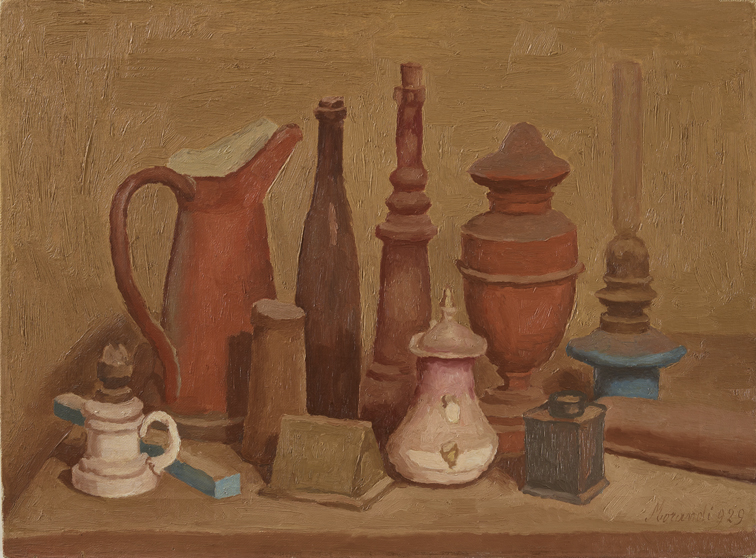
\includegraphics[scale=0.2]{Giorgio Morandi1.jpg}}
			}&{
			\centering
			\zoombox{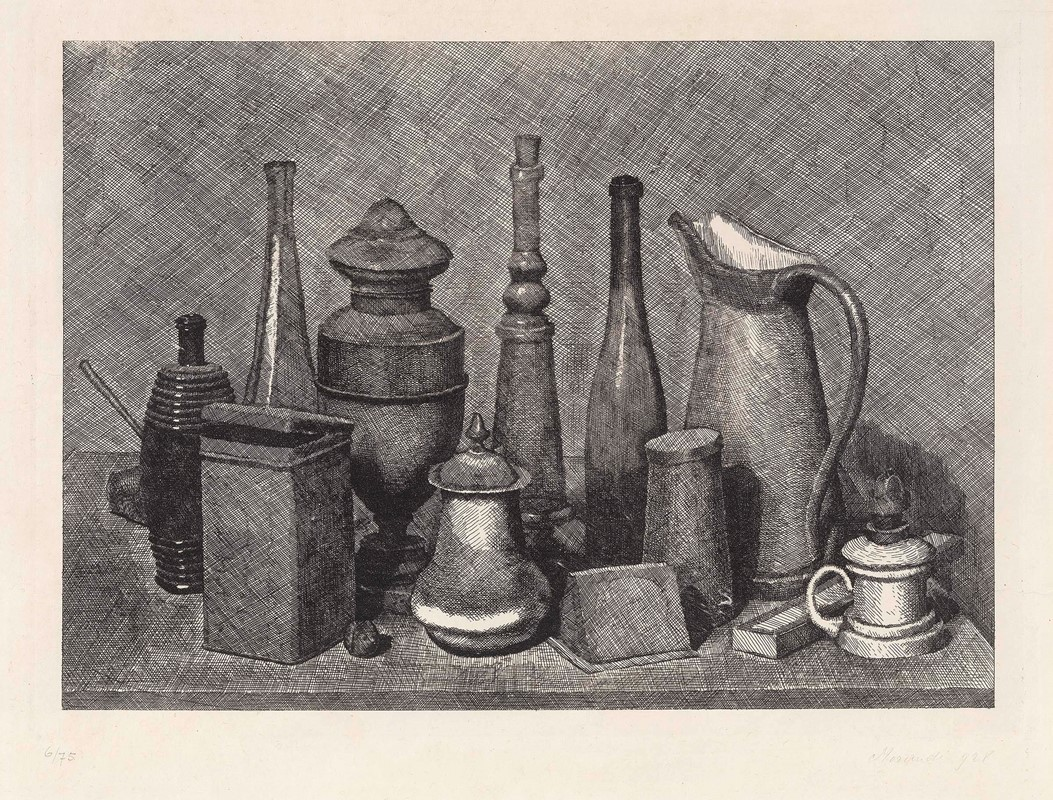
\includegraphics[scale=0.11]{Giorgio Morandi2.jpg}}
			}
		\end{tabularx}
		\centering
		\small{Giorgio Morandi, Grande natura morta}
		\begin{tabularx}{\linewidth}{XX}
				{
				\centering
				\hspace*{40mm}
				\zoombox{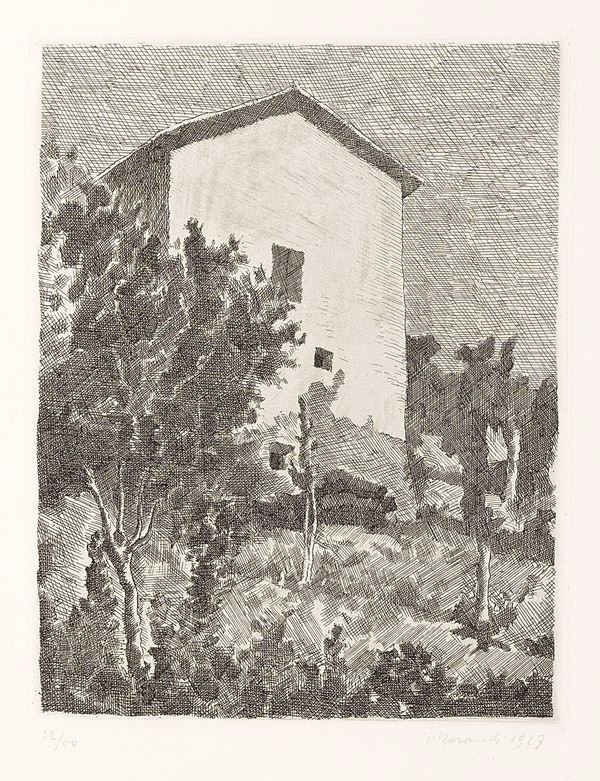
\includegraphics[scale=0.5]{Casolare di Grizzana1.jpg}}
			}&{
				\centering
				\zoombox{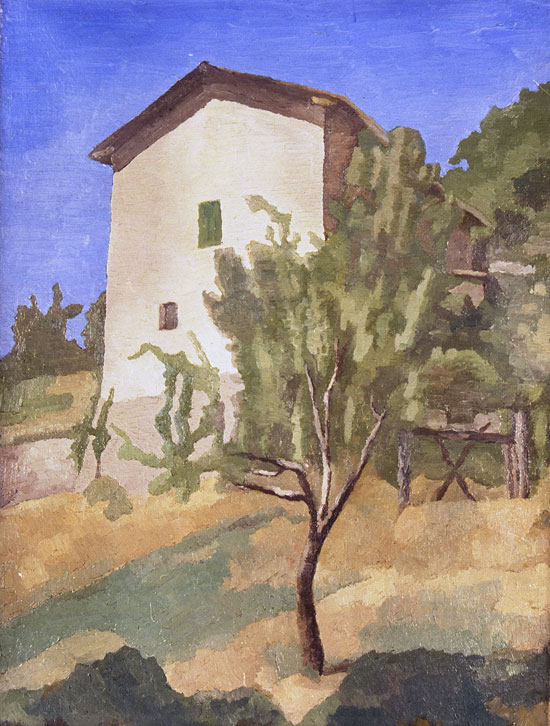
\includegraphics[scale=0.123]{Casolare di Grizzana2.jpg}}
			}
		\end{tabularx}
		\centering
		\small{Casolare di Grizzana, olio su tela e acquaforte}
	\end{frame}
	
	\begin{frame}{Stampa di invenzione (dall'incisione alla pittura e viceversa)}
		\begin{tabularx}{\linewidth}{XX}
			{
			\centering
			\zoombox{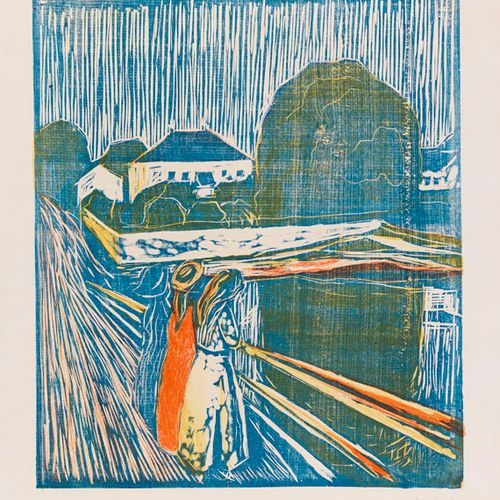
\includegraphics[scale=0.3]{Edvard Munch, Ragazze sul ponte, xilografia.jpg}}
			\captionof{figure}{\centering Edvard Munch, Ragazze sul ponte, xilografia}
			}&{
			\centering
			\zoombox{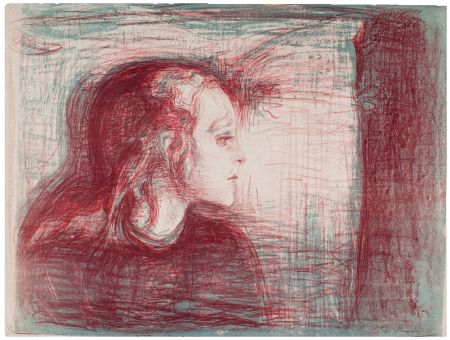
\includegraphics[scale=0.6]{Bambina malata, litografia.jpg}}
			\captionof{figure}{\centering Bambina malata, litografia}
			}
		\end{tabularx}
	\end{frame}
	
	\subsection{Stampa d'après}
	\begin{frame}{Stampa d'après}
		\begin{tabularx}{\linewidth}{XX}
			{
			\centering
			\zoombox{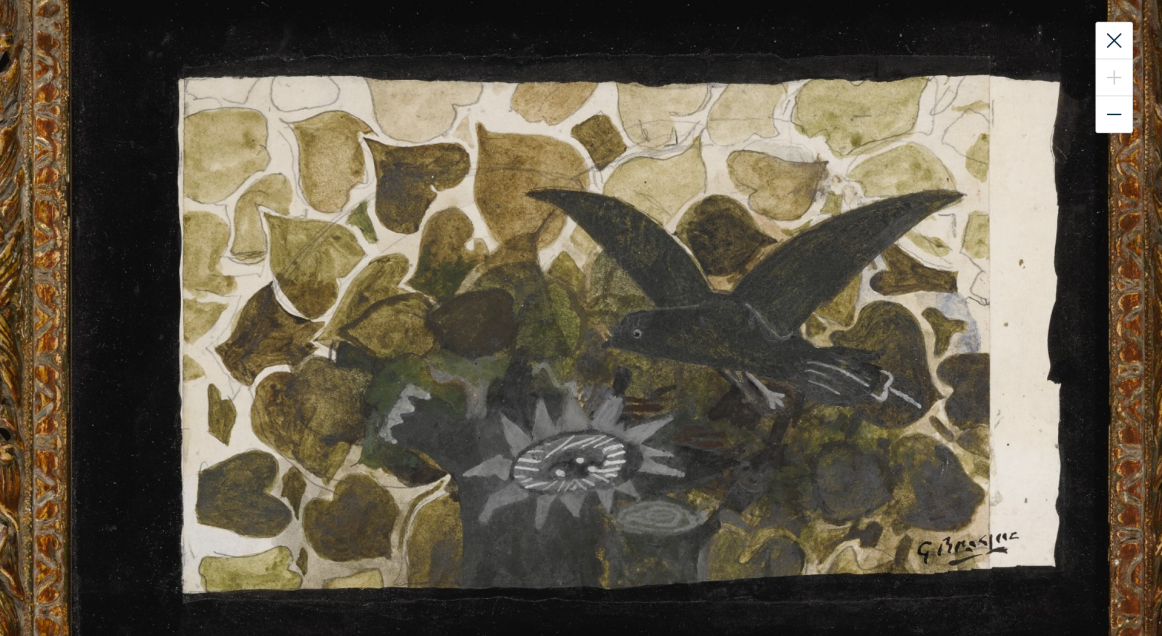
\includegraphics[trim={7mm 3mm 8mm 5mm}, clip, scale=0.6]{George Braque1.png}}
			}&{
			\centering
			\hspace*{15mm}
			\zoombox{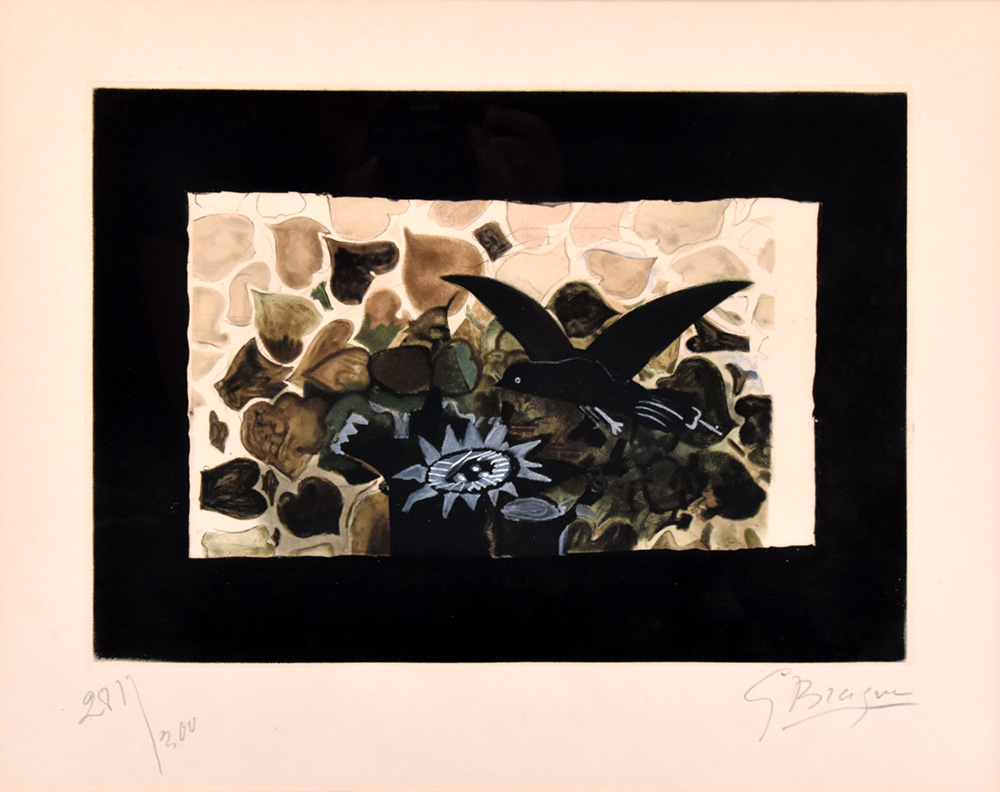
\includegraphics[scale=0.6]{George Braque2.jpg}}
			}
		\end{tabularx}
		\centering
		\small{George Braque, Le nid vert, acquerello, inchiostro e matita su carta – d’aprés acquaforte e acquatinta }
	\end{frame}
	
	\begin{frame}{Stampa d'après}
		\begin{tabularx}{\linewidth}{XX}
			{
			\centering
			\hspace*{20mm}
			\zoombox{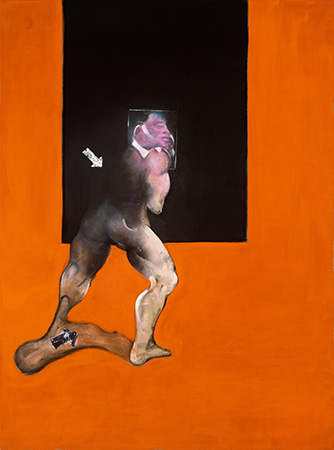
\includegraphics[scale=0.35]{Francis Bacon1.jpg}}
			}&{
			\centering
			\hspace*{10mm}
			\zoombox{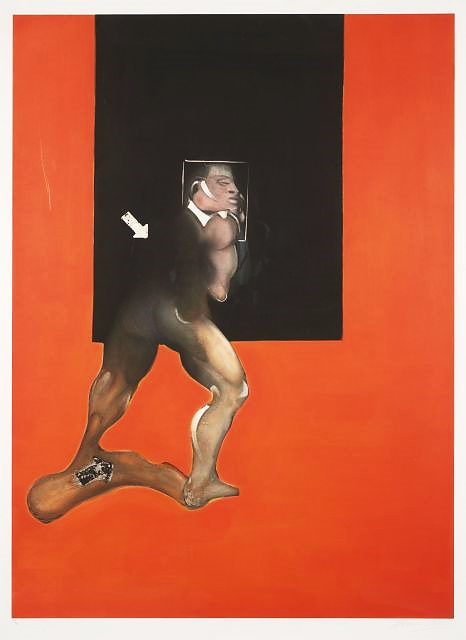
\includegraphics[scale=0.25]{Francis Bacon2.png}}
			}
		\end{tabularx}
		\centering
		\small{Francis Bacon, Studio di corpo umano, olio su tela – d’aprés acquaforte e acquatinta, 2RC Roma}
	\end{frame}
	
	\subsection{Serigrafia fra originalità e riproduzione}
	\begin{frame}{Serigrafia fra originalità e riproduzione}
		\begin{tabularx}{\linewidth}{XX}
			{
			\centering
			\zoombox{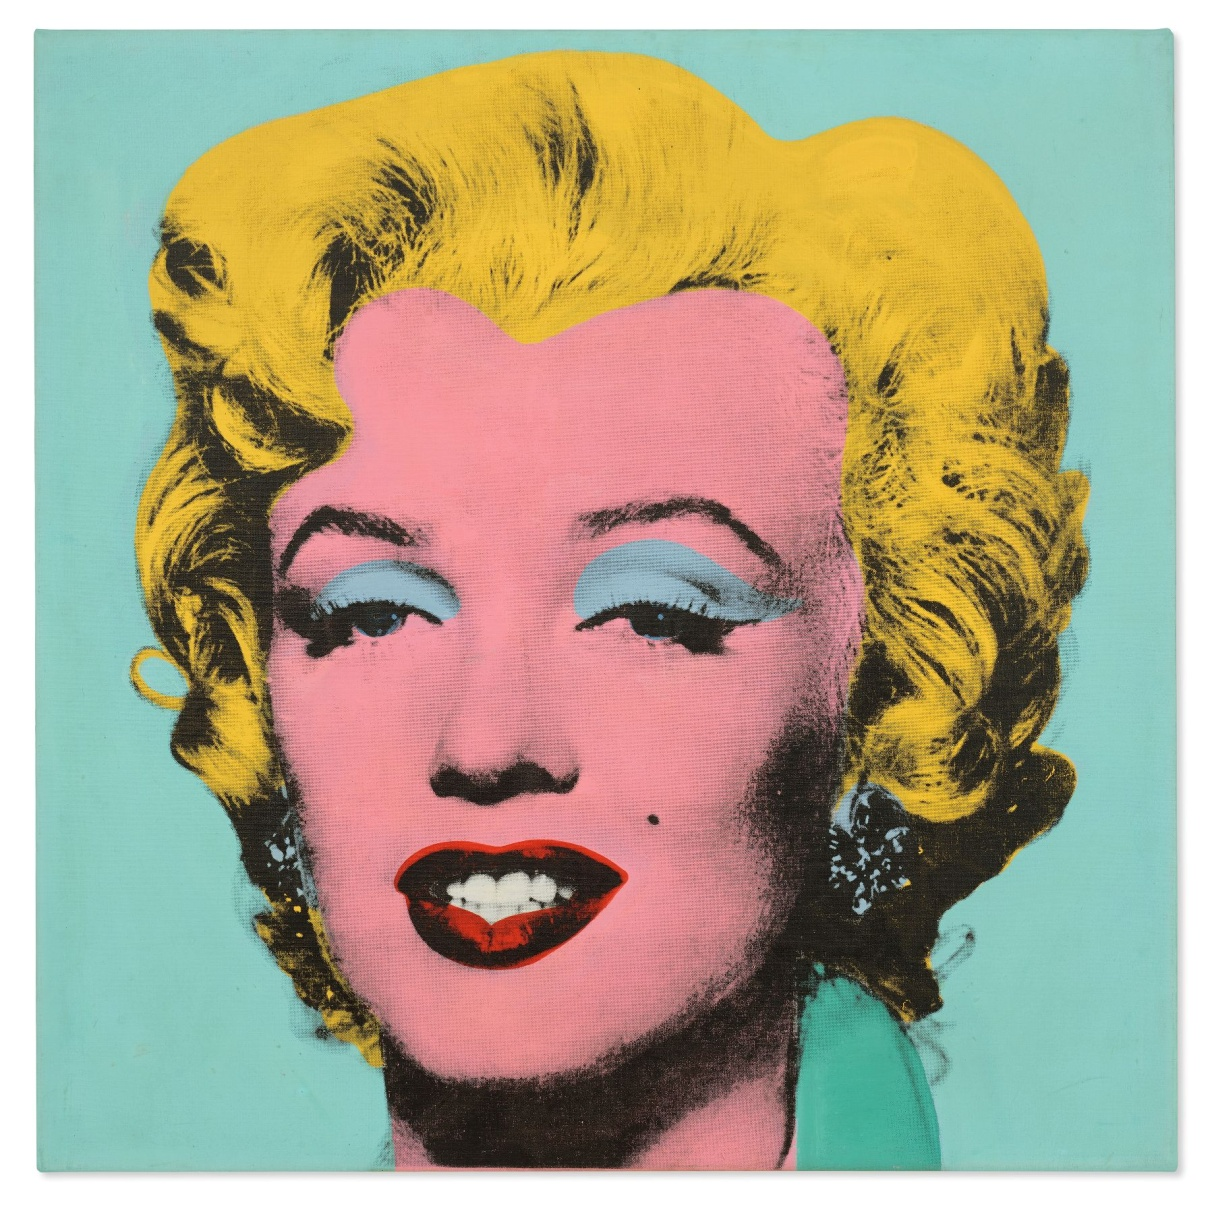
\includegraphics[scale=0.45]{Andy Warhol.jpg}}
			\captionof{figure}{\centering Andy Warhol, Marilyn, serigrafia }
			}&{
			\centering
			\zoombox{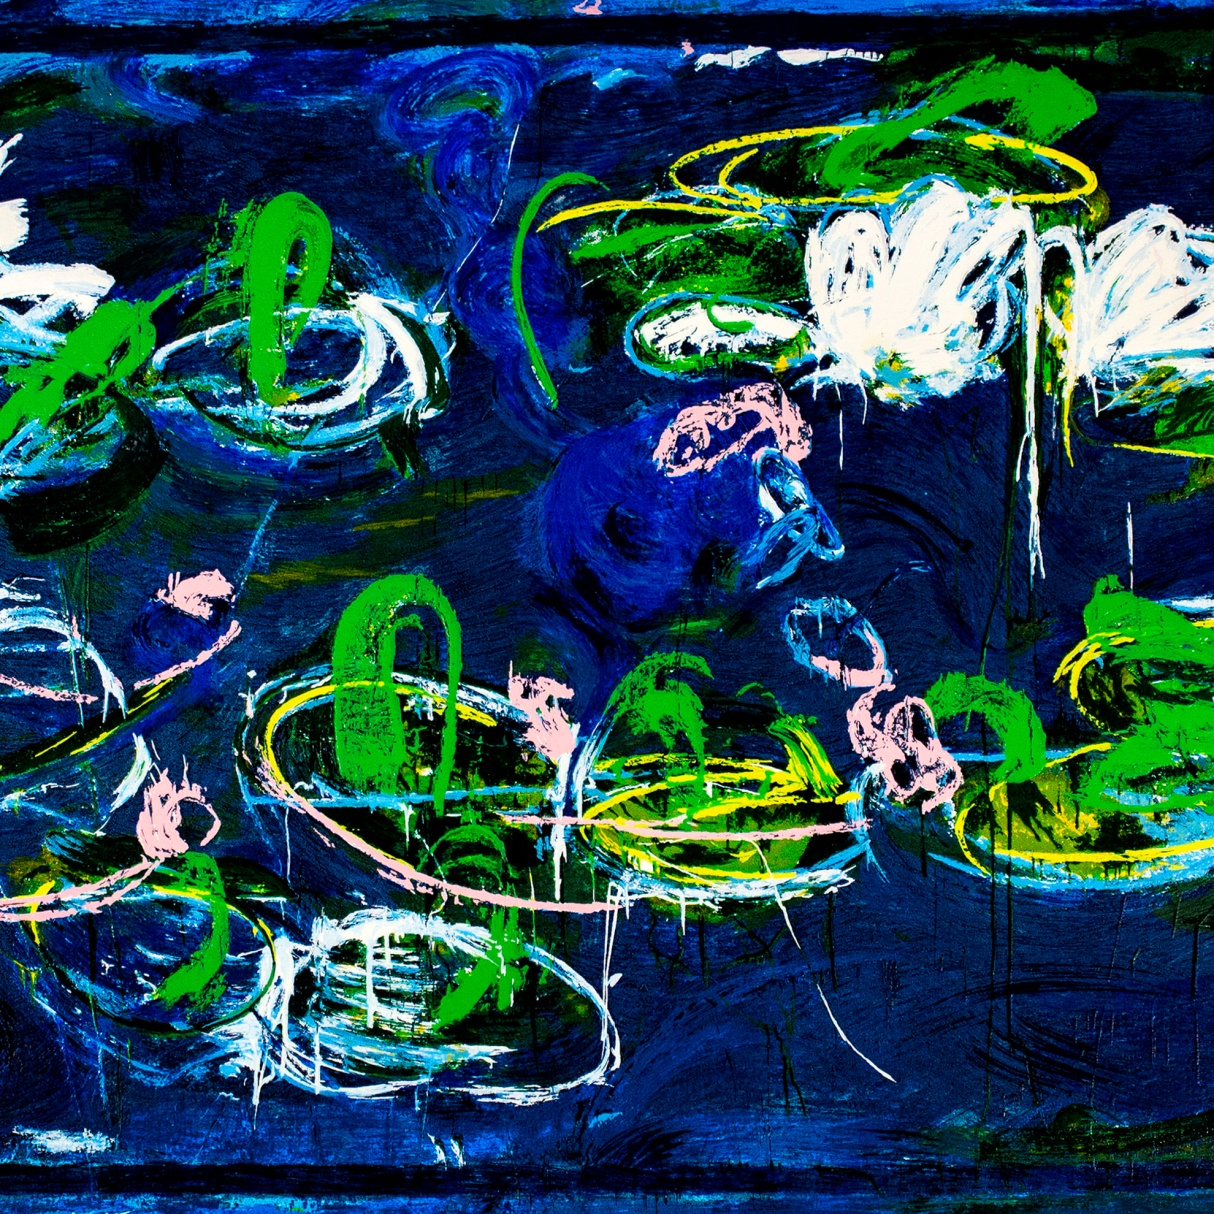
\includegraphics[scale=0.43]{Mario Schifano.jpg}}
			\captionof{figure}{\centering Mario Schifano, I gigli d’acqua, serigrafia}
			}
		\end{tabularx}
	\end{frame}
	
	\subsection{Falso e contraffazione}
	\begin{frame}{Falso e contraffazione}
		\begin{tabularx}{\linewidth}{XX}
			{
			\centering
			\zoombox{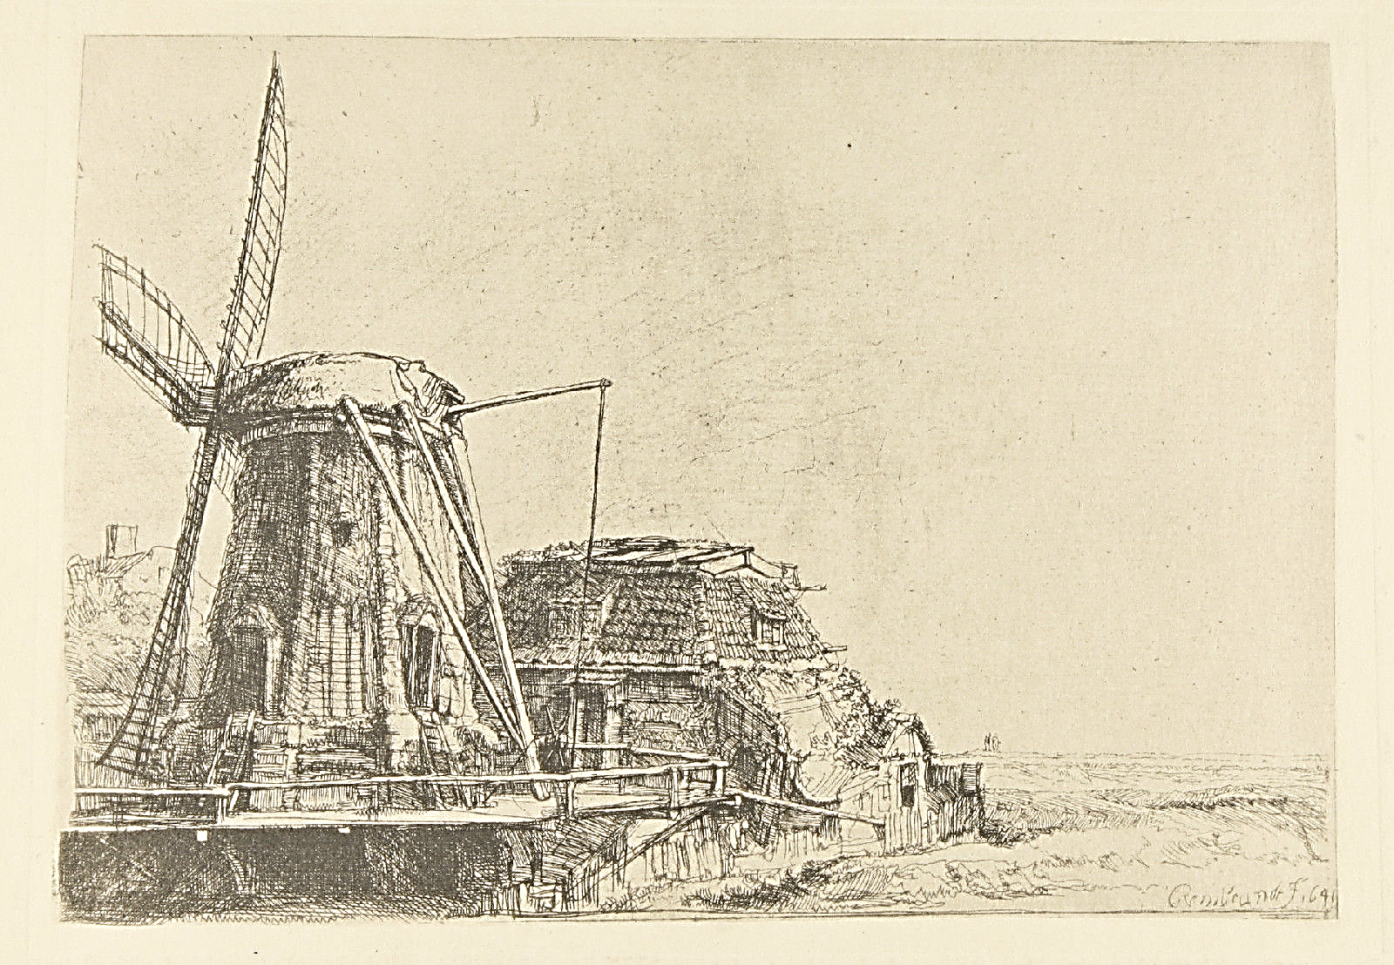
\includegraphics[scale=0.43]{Rembrandt1.png}}
			}&{
			\centering
			\zoombox{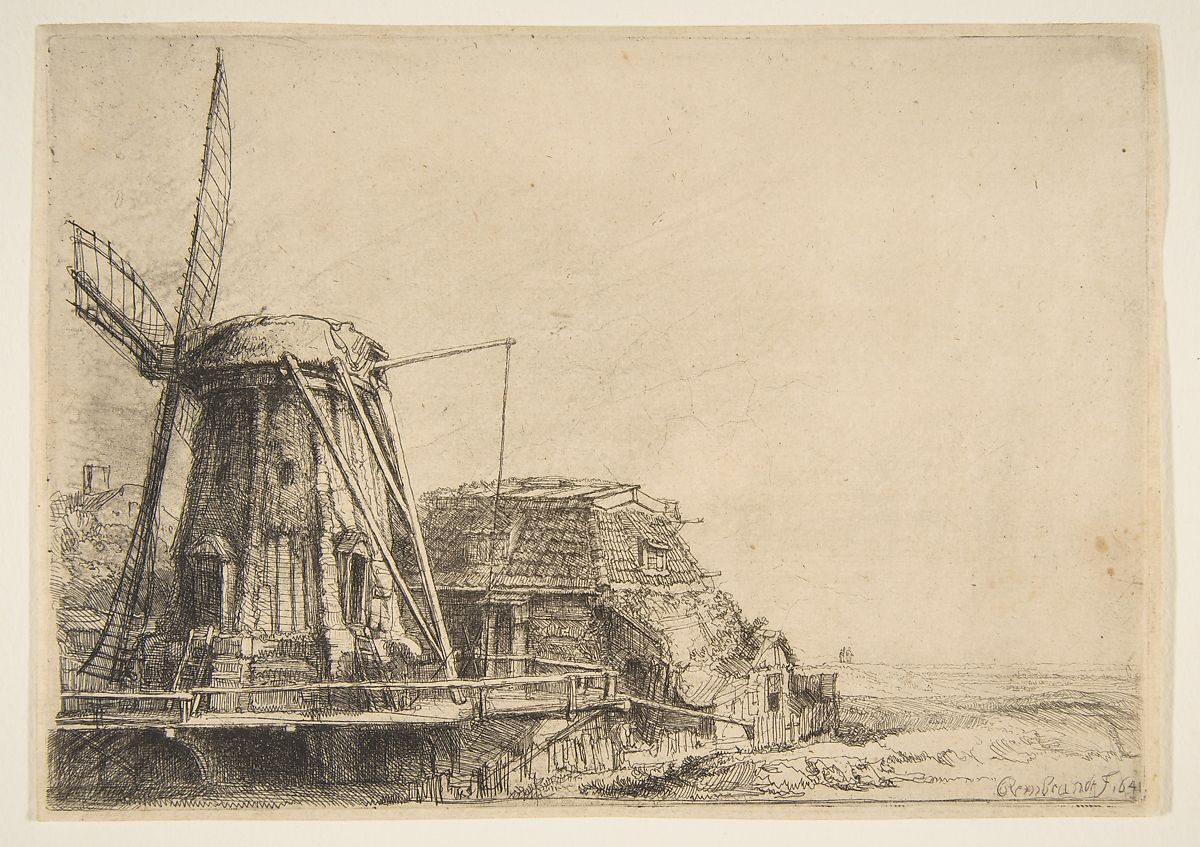
\includegraphics[scale=0.33]{Rembrandt2.jpg}}
			}
		\end{tabularx}
		\centering
		\small{Rembrandt, Il vecchio mulino, acquaforte e puntasecca – da Rembrandt, Il vecchio mulino, copia acquaforte e puntasecca}
	\end{frame}
	
	\begin{frame}{Copia, falso e contraffazione}
		\begin{tabularx}{\linewidth}{XX}
			{
			\centering
			\hspace*{15mm}
			\zoombox{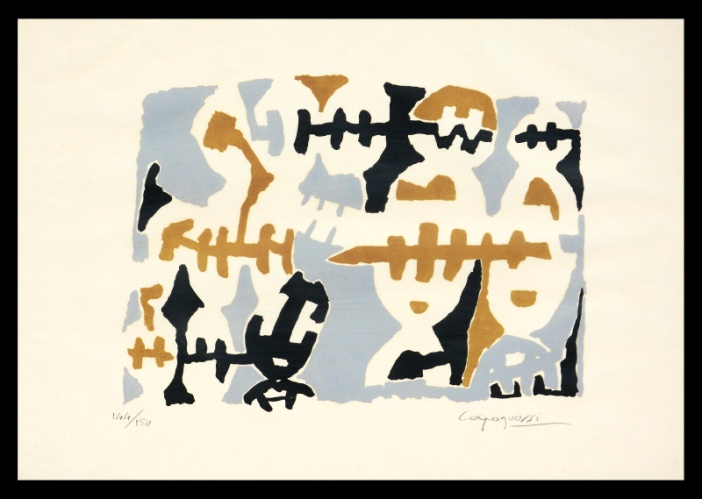
\includegraphics[scale=0.5]{Giuseppe Capogrossi1.png}}
			\newline
			\begin{minipage}{\linewidth}
				\vspace*{2mm}
				\hspace*{15mm}
				\zoombox{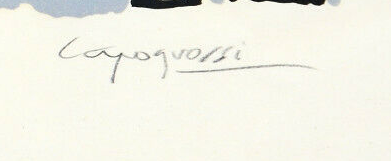
\includegraphics[scale=0.5]{Giuseppe Capogrossi2.png}}
			\end{minipage}
			}&{
			\centering
			\hspace*{5mm}
			\zoombox{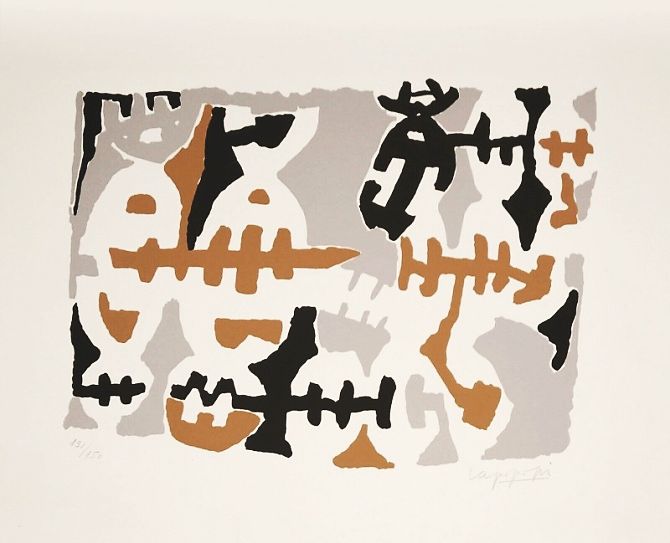
\includegraphics[scale=0.5]{Giuseppe Capogrossi3.png}}
			\newline
			\begin{minipage}{\linewidth}
				\vspace*{2mm}
				\hspace*{5mm}
				\zoombox{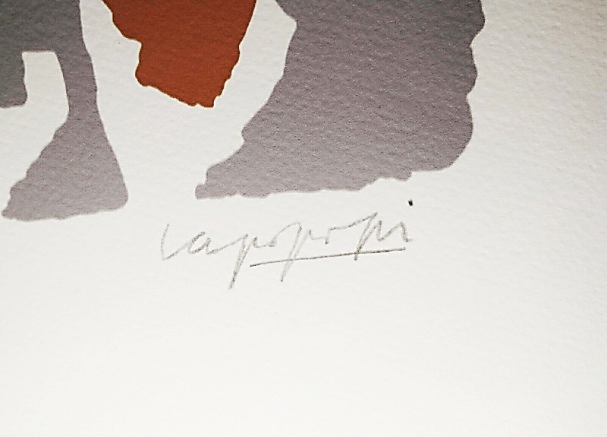
\includegraphics[scale=0.5]{Giuseppe Capogrossi4.png}}
			\end{minipage}
			}
		\end{tabularx}
		\begin{minipage}{\linewidth}
			\vspace*{2mm}
			\centering
			\small{Da Giuseppe Capogrossi, litografia (capovolta) – Giuseppe Capogrossi, litografia}
		\end{minipage}
	\end{frame}
	
	\subsection{Varianti di stato}
	\begin{frame}{Varianti di stato}
		\begin{tabularx}{\linewidth}{XXXX}
			{
			\centering
			\zoombox{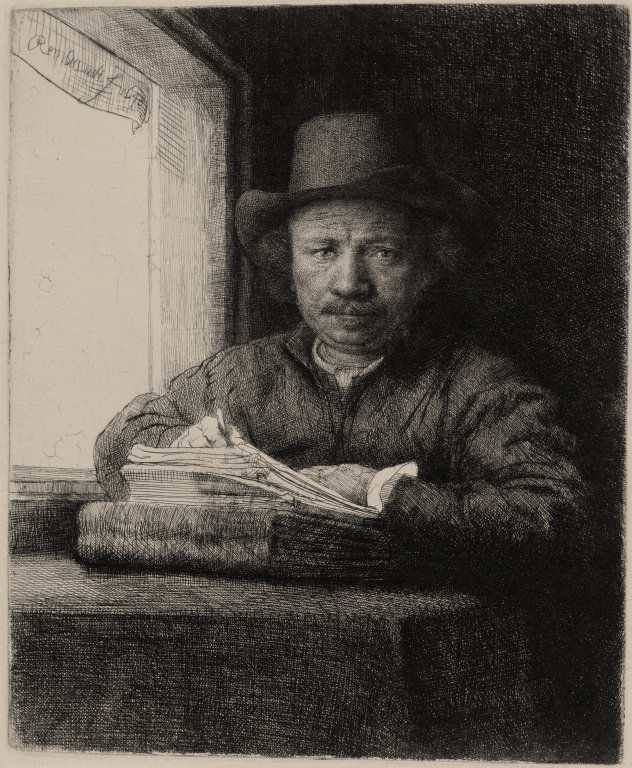
\includegraphics[scale=0.2]{Rembrandt3.png}}
			}&{
			\centering
			\zoombox{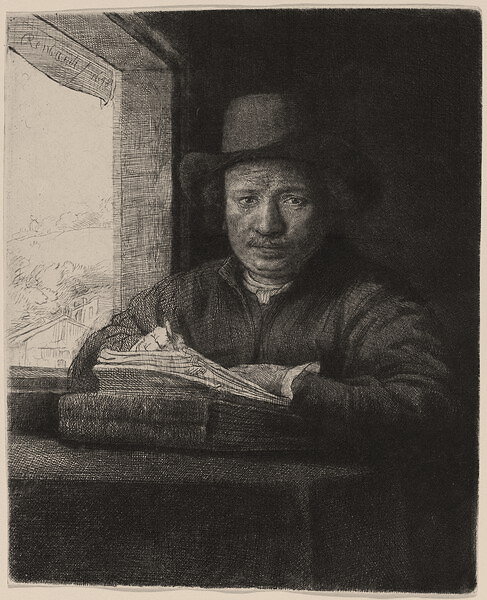
\includegraphics[scale=0.25]{Rembrandt4.png}}
			}&{
			\centering
			\zoombox{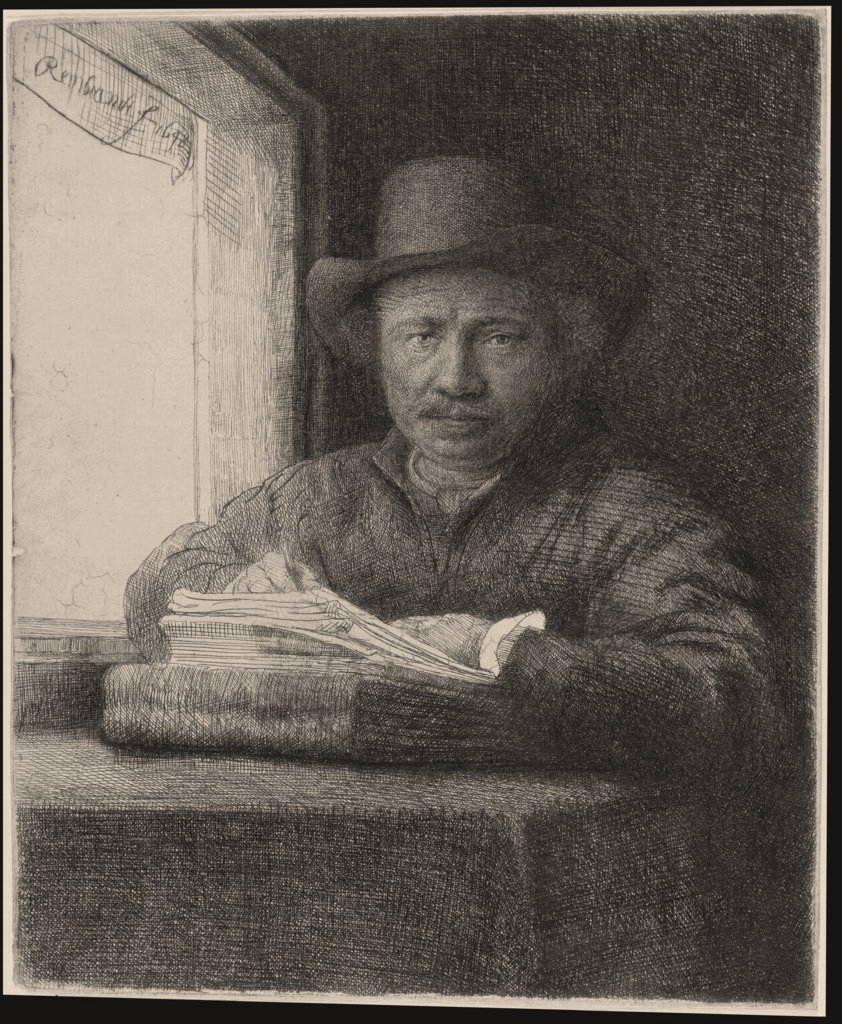
\includegraphics[scale=0.15]{Rembrandt5.png}}
			}&{
			\vspace*{-30mm}
			\begin{flushleft}
					\small{Rembrandt, Autoritratto alla finestra, acquaforte e puntasecca nei vari stati}
			\end{flushleft}
			}
		\end{tabularx}
		\begin{tabularx}{\linewidth}{XXXX}
			{
			\centering
			\zoombox{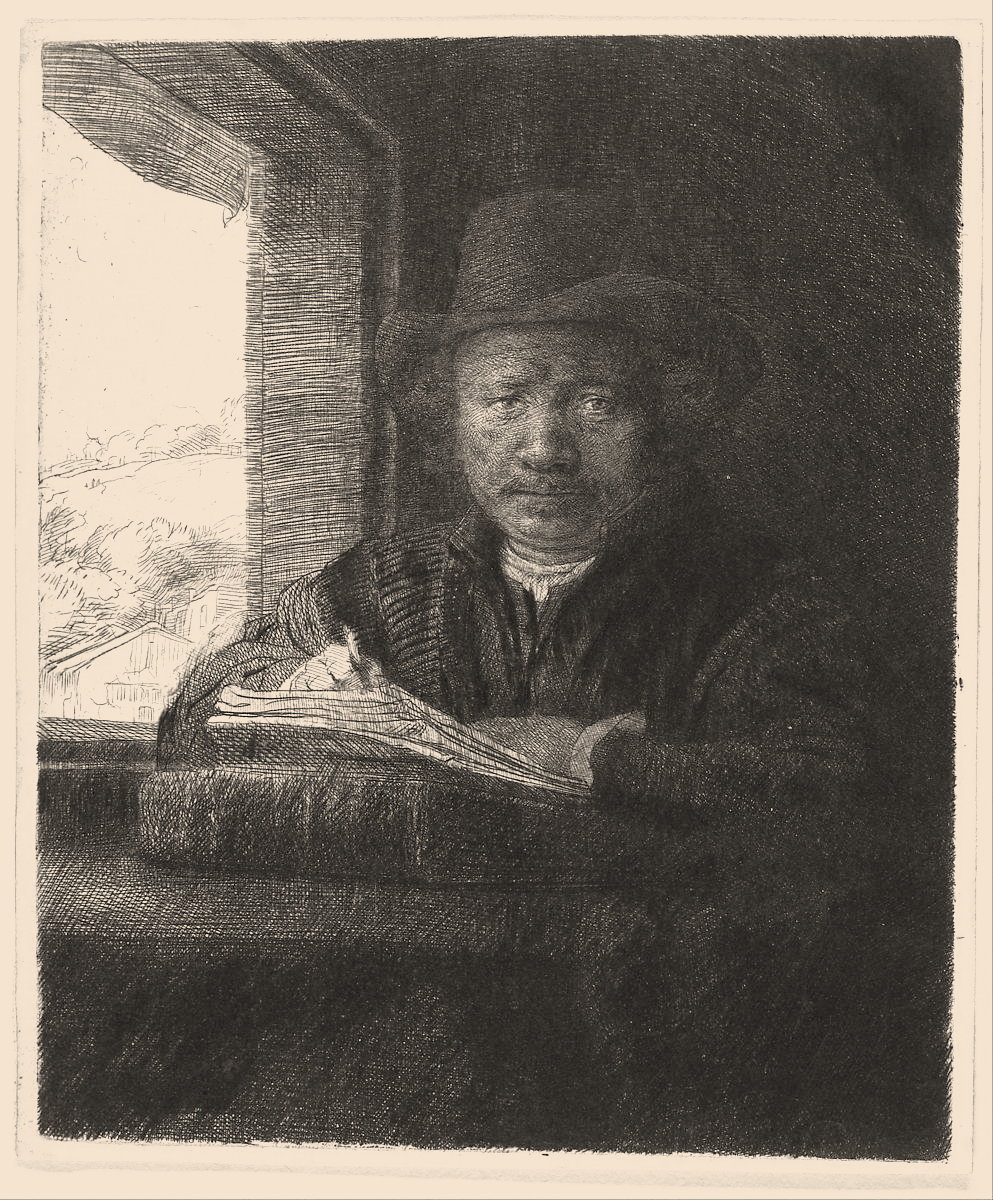
\includegraphics[scale=0.13]{Rembrandt6.png}}
			}&{
			\centering
			\zoombox{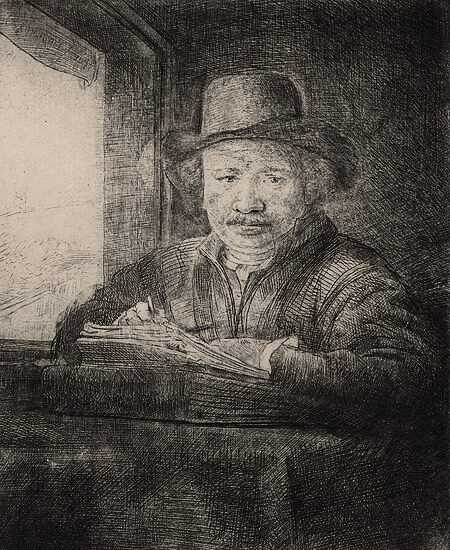
\includegraphics[scale=0.27]{Rembrandt7.png}}
			}&{
			\centering
			\zoombox{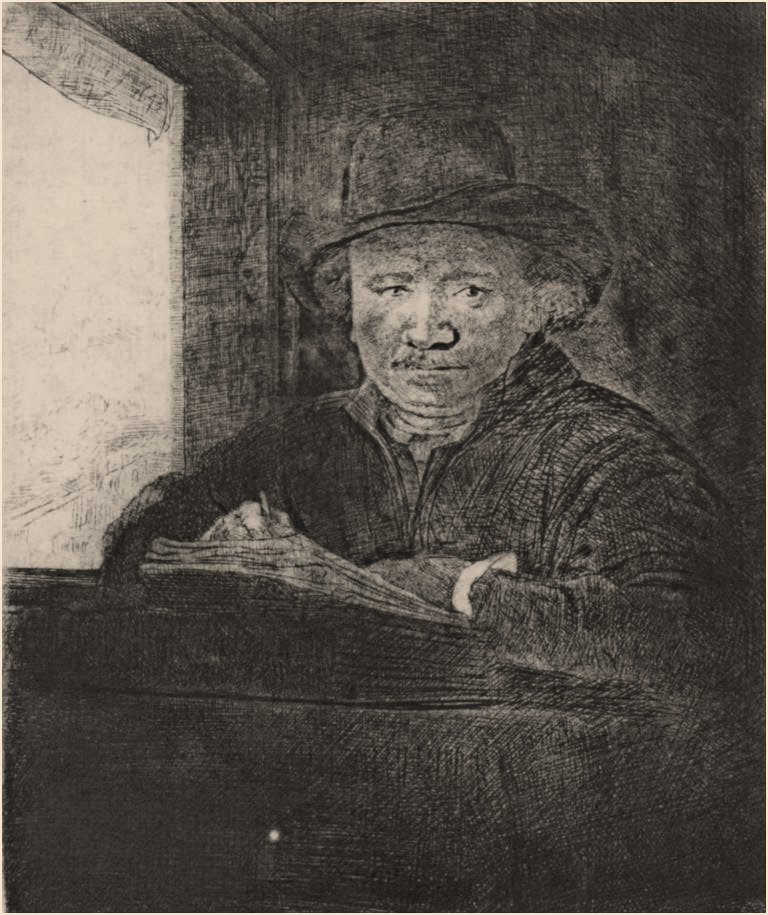
\includegraphics[scale=0.165]{Rembrandt8.png}}
			}&{
			}
		\end{tabularx}
		
	\end{frame}
	
	\begin{frame}{Varianti di stato}
		\begin{tabularx}{\linewidth}{XXXX}
			{
			\centering
			\zoombox{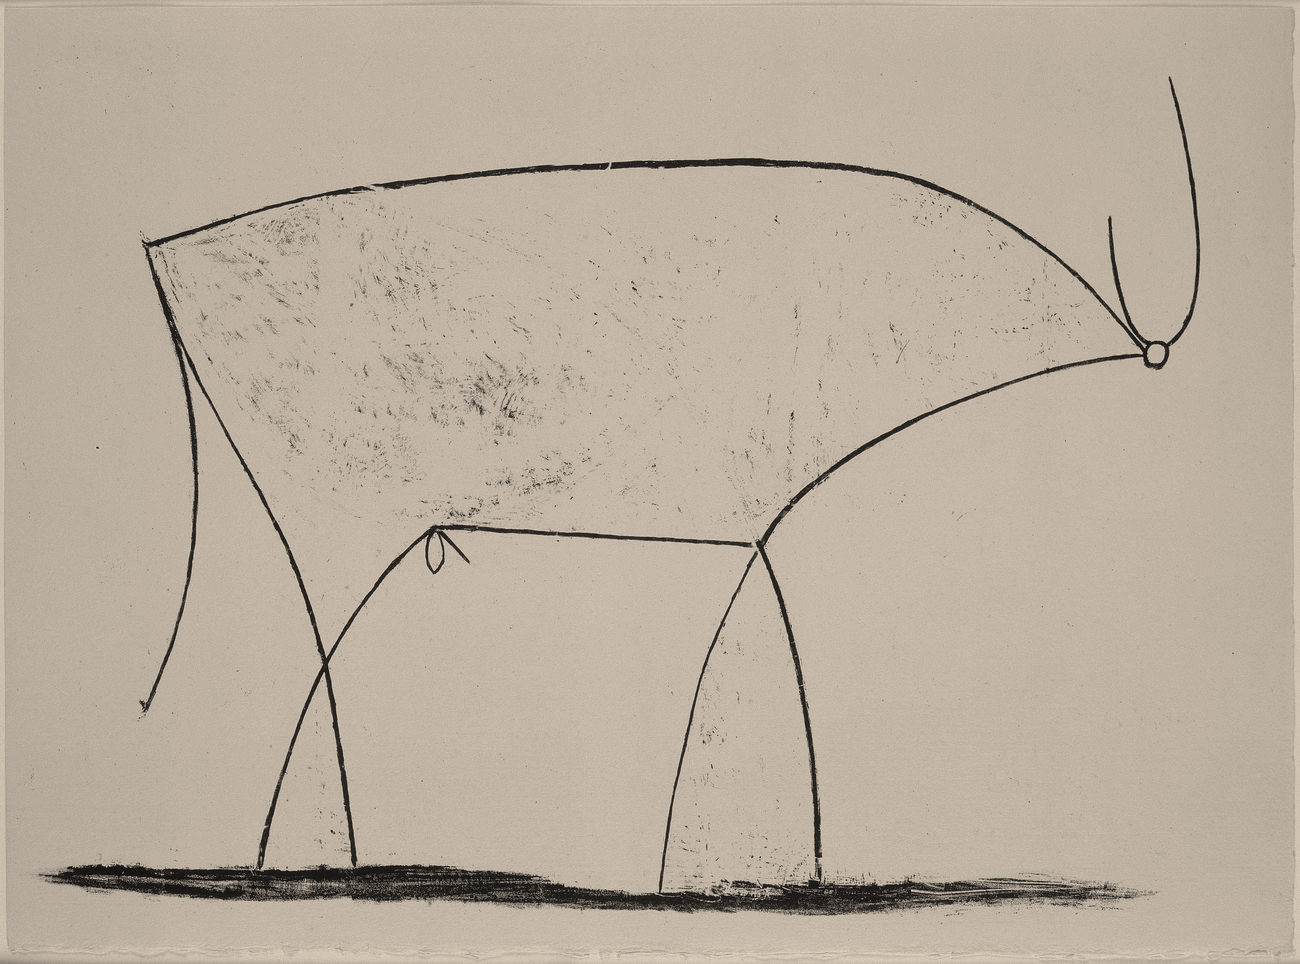
\includegraphics[scale=0.08]{Pablo Picasso1.png}}
			}&{
			\centering
			\zoombox{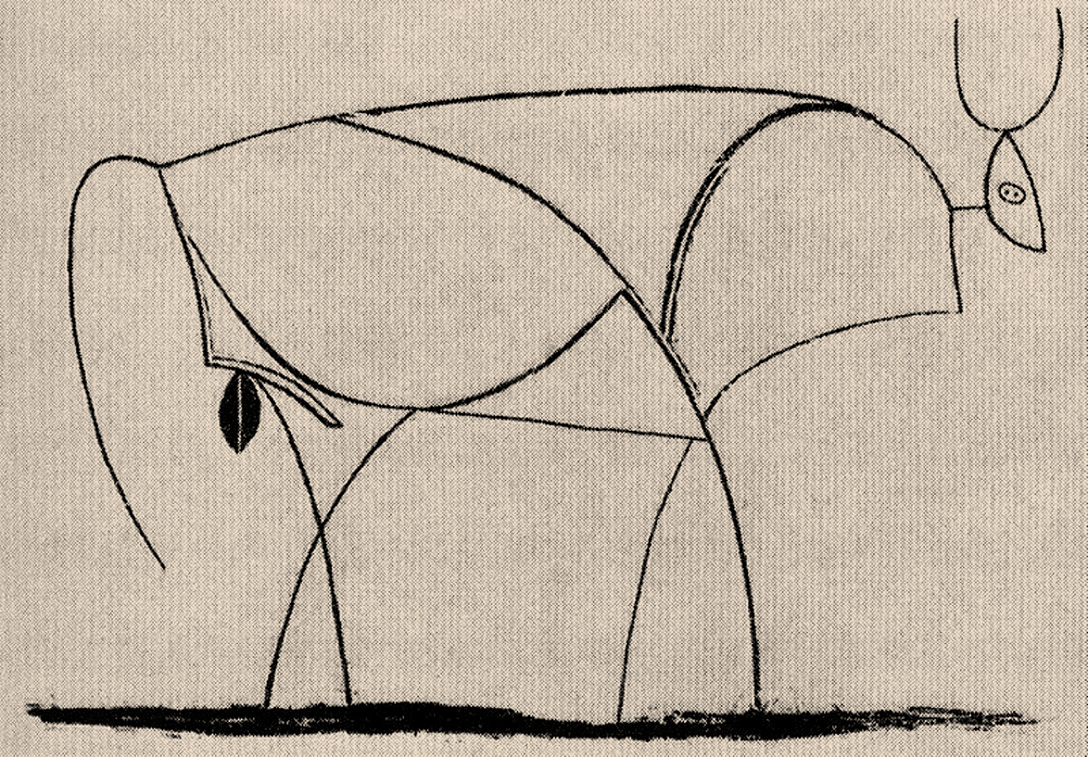
\includegraphics[scale=0.1]{Pablo Picasso2.png}}
			}&{
			\centering
			\zoombox{\includegraphics[scale=0.18]{Pablo Picasso3.png}}
			}&{
			\centering
			\zoombox{\includegraphics[scale=0.18]{Pablo Picasso4.png}}
			}
		\end{tabularx}
		\begin{tabularx}{\linewidth}{XXXX}
			{
			\centering
			\zoombox{\scalebox{-1}[1]{\includegraphics[scale=0.08]{Pablo Picasso5.png}}}
			}&{
			\centering
			\zoombox{\includegraphics[scale=0.45]{Pablo Picasso6.png}}
			}&{
			\centering
			\zoombox{\includegraphics[scale=0.15]{Pablo Picasso7.png}}
			}&{
			\centering
			\zoombox{\includegraphics[scale=0.14]{Pablo Picasso8.png}}
			}
		\end{tabularx}
		\begin{tabularx}{\linewidth}{XXXX}
			{
			\centering
			\zoombox{\includegraphics[scale=0.1]{Pablo Picasso9.png}}
			}&{
			\centering
			\zoombox{\includegraphics[scale=0.45]{Pablo Picasso10.png}}
			}&{
			\centering
			\zoombox{\includegraphics[scale=0.1]{Pablo Picasso11.png}}
			}&{
			\vspace*{-20mm}
			\begin{flushleft}
				\small{Pablo Picasso, Toro, litografia negli undici stati}
			\end{flushleft}
			}
		\end{tabularx}
	\end{frame}
	
\end{document}